\documentclass[11pt,twoside]{book}
\usepackage[utf8]{inputenc}
\usepackage[spanish]{babel}
%%%%%%%%%%%%%%%%%%%%%%%%%%%%%%%%%%%%%%%%%%%%%%%%%%%%%%%%%%%%%%%%%%%%%%%%%%%%%%%%%%%%%%%%%%%%%%%%%%%%%%%
\usepackage{afterpage}% Necesario para introdicur páginas A3
\usepackage{amsmath,amsthm,amstext,amssymb}
\usepackage{capt-of}
\usepackage{colortbl}
\usepackage{graphicx}% Permite la introducción de figuras
\usepackage{array,fancyhdr,graphicx,subfigure,titlesec,titletoc,xcolor}
\usepackage{emptypage}% evita la numeración de las páginas en blanco
\usepackage{etoolbox}
\usepackage{listings} % premite la introducción de códigos vhdl
\usepackage[paper=A4,pagesize]{typearea}%necesario para introducir páginas A3
\usepackage{lscape}% Necesario para páginas apaisadas
\usepackage{pdfpages}% Permite introducir documentos pdf
\usepackage[font=small,bf]{caption}% Formato del caption
\usepackage{rotating}% Rotaciones
\usepackage{setspace,subfigure}
\usepackage{tocstyle}
\usepackage{codigomatlab}
\usepackage{titlesec}
\usepackage{color}
\usepackage{tikz}
\usetikzlibrary{calc}
\usepackage{pstricks}
\usepackage{pst-node}
\usepackage{pst-blur}
\usepackage{amsmath,amssymb}
\usepackage{booktabs}
\usepackage{xcolor}
\usepackage{colortbl}
\usepackage{rotating}
\usepackage{multirow}
\usepackage{bigstrut}
\usepackage{eurosym}
%\usepackage{inputenc}
%%%%%%%%%%%%%%%%%%%%%%%%%%%%%%%%%%%%%%%%%%%%%%%%%%%%%%%%%%%%%%%%%%%%%%%%%%%%%%%%%%%%%%%%%%%
\newcommand{\documento}{ÍÍNDICE XERAL}
%%%%%%%%%%%%%%%%%%%%%%%%%%%%%%%%%%%%%%%%%%%%%%%%%%%%%%%%%%%%%%%%%%%%%%%%%%%%%%%%%%%%%%%%%%%
% Incluye la bibliografía como sección
\makeatletter
\renewenvironment{thebibliography}[1]
     {\chapter{\bibname}% esta línea cambia la bibliografía a la categoría sección
      \@mkboth{\MakeUppercase\bibname}{\MakeUppercase\bibname}
      \list{\@biblabel{\@arabic\c@enumiv}}%
           {\settowidth\labelwidth{\@biblabel{#1}}
            \leftmargin\labelwidth
            \advance\leftmargin\labelsep
            \@openbib@code
            \usecounter{enumiv}
            \let\p@enumiv\@empty
            \renewcommand\theenumiv{\@arabic\c@enumiv}}
      \sloppy
      \clubpenalty4000
      \@clubpenalty \clubpenalty
      \widowpenalty4000%
      \sfcode`\.\@m}
     {\def\@noitemerr
       {\@latex@warning{Empty `thebibliography' environment}}
      \endlist}
\makeatother
%%%%%%%%%%%%%%%%%%%%%%%%%%%%%%%%%%%%%%%%%%%%%%%%%%%%%%%%%%%%%%%%%%%%%%%%%%%%%%%%%%%%%%%%%%%%%%%%%%%%%%%%%%%%%%%%%%%%%%%%%%%%%%%%%%%%%%%%%%%%%%%%%%%%%%%%%%%%%%%%%%%%%
%FORMATO DE LA HOJA
\renewcommand{\baselinestretch}{1.25}
\headsep 8mm        \topmargin -1.5cm     \textheight 24.5cm     \textwidth 16cm     \oddsidemargin 0.5cm     \evensidemargin -0.1cm
 \footnotesep=20pt               \footskip=38pt
%%%%%%%%%%%%%%%%%%%%%%%%%%%%%%%%%%%%%%%%%%%%%%%%%%%%%%%%%%%%%%%%%%%%%%%%%%%%%%%%%%%%%%%%%%%%%%%%%%%%%%%%%%%%%%%%%%%%%%%%%%%%%%%%%%%%%%%%%%%%%%%%%%%%%%%%%%%%%%%%%%%%%
% Formato del título de cada parte
\titleformat{\part}[display]
  {\normalfont\huge\bfseries}
	{}{0pt}{\centering}
	
\titlespacing*{\part}{0pt}{0pt}{20pt}
\titleclass{\part}{straight}
%%%%%%%%%%%%%%%%%%%%%%%%%%%%%%%%%%%%%%%%%%%%%%%%%%%%%%%%%%%%%%%%%%%%%%%%
%Formato del título de cada capítulo
\titleformat{\chapter}[hang] 
{\normalfont\huge\bfseries}{\thechapter}{1em}{} 
%%%%%%%%%%%%%%%%%%%%%%%%%%%%%%%%%%%%%%%%%%%%%%%%%%%%%%%%%%%%%%%%%%%%%%%%
% Espacio vertical en TOC
%\makeatletter
%\pretocmd{\part}{\addtocontents{toc}{\protect\addvspace{10\p@}}}{}{}
%\pretocmd{\chapter}{\addtocontents{toc}{\protect\addvspace{2\p@}}}{}{}
%\makeatother
%%%%%%%%%%%%%%%%%%%%%%%%%%%%%%%%%%%%%%%%%%%%%%%%%%%%%%%%%%%%%%%%%%%%%%
%Formato de letra
\usepackage{lmodern}
\renewcommand*\familydefault{\sfdefault} %% Only if the base font of the document 
%%%%%%%%%%%%%%%%%%%%%%%%%%%%%%%%%%%%%%%%%%%%%%%%%%%%%%%%%%%%%%%%%%%%%%%%%%%%%%%%%%%%%%%%%%%%
\renewcommand{\spanishtablename}{Tabla}% escribe Tabla
%\renewcommand*\listtablename{Índice de tablas}
%\renewcommand{\contentsname}{Contidos do PFG}
%%%%%%%%%%%%%%%%%%%%%%%%%%%%%%%%%%%%%%%%%%%%%%%%%%%%%%%%%%%%%%%%%%%%%%%%%%%%%%%%
\setcounter{secnumdepth}{5}% Profundidad del índice de contenidos
%%%%%%%%%%%%%%%%%%%%%%%%%%%%%%%%%%%%%%%%%%%%%%%%%%%%%%%%%%%%%%%%%%%%%%%%%%%%%%%%%%%%%%%%%%%%%%%%%%%%%%%%%%%%%%%%%%%%%%%%%%%%%%%%%%%%%%%%%%%%%%%%%%%%%%%%%%%%%%%%%%%%%%%%%%%%%
\numberwithin{equation}{subsection}
\usepackage{chngcntr}
\counterwithin{table}{subsection}% Numera las tablas por sucsecciones
\counterwithin{figure}{subsection}% Numera las figuras por sucsecciones

\DeclareCaptionLabelSeparator{guion}{\ --\ }
\captionsetup[figure]{labelsep=guion}% establece un guión como separador en el pie de figura
\captionsetup[table]{labelsep=guion}% establece un guión como separador en el pie de tabla
%%%%%%%%%%%%%%%%%%%%%%%%%%%%%%%%%%%%%%%%%%%%%%%%%%%%%%%%%%%%%%%%%%%%%%%%%%%%%%%%%%%%%%%%%%%%%%%%%%%%%%%%%%%%%%%%%%%%%%%%%%%%%%%%%%%
\usepackage{float}
\newfloat{Plano}{p}{pln}%[chapter]
\captionsetup[Plano]{labelformat=empty,labelsep=none,position=below}
%%%%%%%%%%%%%%%%%%%%%%%%%%%%%%%%%%%%%%%%%%%%%%%%%%%%%%%%%%%%%%%%%%%%%%%%%%%%%%%%%%%%%%%%%%%%%%%%%%%%%%%%%%%%%%%%%%%%%%%%%%%%%%%%%%%%%%%%%%%%%
\usepackage{float}
\newfloat{Circuito}{c}{cir}%[chapter]
\captionsetup[Circuito]{labelformat=empty,labelsep=none}
%%%%%%%%%%%%%%%%%%%%%%%%%%%%%%%%%%%%%%%%%%%%%%%%%%%%%%%%%%%%%%%%%%%%%%%%%%%%%%%%%%%%%%%%%%%%%%%%%%%%%%%%%%%%%%%%%%%%%%%%%%%%%%%%%%%%%%%%%%%%%
\usepackage[subfigure]{tocloft}% Permite cambiar el ancho de la numeración de listas de figuras y tablas
\addtolength{\cfttabnumwidth}{17pt}
\addtolength{\cftfignumwidth}{17pt}
\makeatletter
\let\l@lstlisting\l@figure
\makeatother
%%%%%%%%%%%%%%%%%%%%%%%%%%%%%%%%%%%%%%%%%%%%%%%%%%%%%%%%%%%%%%%%%%%%%%%%%%%%%%%%%%%%%%%%%%%%%%%%%%%%%%%%%%%%%%%%%%%%%%%%%%%%%%%%%%%%%%%%%%
\patchcmd{\chapter}{plain}{fancy}{}{}% Permite que el formato de la primera página sea como los demás
%%%%%%%%%%%%%%%%%%%%%%%%%%%%%%%%%%%%%%%%%%%%%%%%%%%%%%%%%%%%%%%%%%%%%%%%%%%%%%%%%%%%%%%%%%%%%%%%%%%%%%%%%%%%%%%%%%%%%%%%%%%%%%%%%%%%%%%%%%
\AtBeginDocument{\addtocontents{toc}{\protect\thispagestyle{fancy}}} % Permite que el formato de la página de tableofcontents sea como los demás
%%%%%%%%%%%%%%%%%%%%%%%%%%%%%%%%%%%%%%%%%%%%%%%%%%%%%%%%%%%%%%%%%%%%%%%%%%%%%%%%%%%%%%%%%%%%%%%%%%%%%%%%%%%%%%%
% Uso de las cabeceras fancy
\fancyhf{}
\fancyfoot[R]{\small \thepage}
\fancyfoot[C]{\small \raisebox{0pt}{\documento}}
\fancyhead[L]{\small \titulouno \ \\ \alumno}
% Introducir la especialidad-----------------------------------------------------------------------------------------------------
\fancyhead[C]{}% Escribir ELECTRICIDAD o ELECTRÓNICA                                                         -
% Introducir el número del PFG---------------------------------------------------------------------------------------------------
\fancyhead[R]{}% E es la especialidad 1=Electrónica 2=Electricidad   XXX es el número del proyecto     -
% Introducir la convocatoria del PFG---------------------------------------------------------------------------------------------
\fancyfoot[L]{}% Por ejemplo JUNIO 2014

\renewcommand{\headrulewidth}{0.5pt}
\renewcommand{\footrulewidth}{0.5pt}
%%%%%%%%%%%%%%%%%%%%%%%%%%%%%%%%%%%%%%%%%%%%%%%%%%%%%%%%%%%%%%%%%%%%%%%%%%%%%%%%%%%%%%%%%%%%%%%%%%%%%%%%%%%%%%%%%%%%%%%%%%%%%%%
% Paquete hyperref
\usepackage[colorlinks=true,linkcolor=red,citecolor=red,urlcolor=red]{hyperref}
%%%%%%%%%%%%%%%%%%%%%%%%%%%%%%%%%%%%%%%%%%%%%%%%%%%%%%%%%%%%%%%%%%%%%%%%%%%%%%%%%%%%%%%%%%%%%%%%%%%%
% Se cambio el nombre del caption para los códigos
\renewcommand\lstlistingname{Código}
%%%%%%%%%%%%%%%%%%%%%%%%%%%%%%%%%%%%%%%%%%%%%%%%%%%%%%%%%%%%%%%%%%%%%%%%%%%%%%%%%%%%%%%%%%%%%%%%%%%%%%%%%%%%%%%%%%%%%%%%%%%%%%%%%%
%  Permite meter figuras partidas en páginas
\newcommand\Image[3][]{
  \tabular[b]{@{}c@{}}\includegraphics[#1]{#2}\\
    {\small #3}
  \endtabular}
%%%%%%%%%%%%%%%%%%%%%%%%%%%%%%%%%%%%%%%%%%%%%%%%%%%%%%%%%%%%%%%%%%%%%%%%%%%%%%%%%%%%%%%%%%%%%%%%%%%%%%%%%%%%%%%%%%%%%%%%%%%%%%%%%%




%%%%%%%%%%%%%%%%%%%%%%%%%%%%%%%%%%%%%%%%%%%%%%%%%%%%%%%%%%%%%%%%%%%%%%%%%%%%%%%%%%%%%%%%%%%%%%%%%%%%%%%%%
%%%%%%%%%%%%%%%%%%%%%%%%%%%%%%%%%%%%%%%%%%%%%%%%%%%%%%%%%%%%%%%%%%%%%%%%%%%%%%%%%%%%%%%%%%%%%%%%%%%%%%%%%
%--------------------------------------------------------------------------------------------------------
%             Datos del ALUMNO
%--------------------------------------------------------------------------------------------------------
\newcommand{\alumno}{
% 1 Se debe introducir el NOMBRE y APELLIDOS del alumno (EN MAY�SCULAS)
Ávaro Fernádez Quesada
}
\newcommand{\especialidad}{
% 2 Introducir LA ESPECIALIDAD: ELECTR�NICA o ELECTRICA
Grao en Enxeñeríaren Electrónica Industrial e Automática
}
\newcommand{\grado}{
% 3 Introducir el grado: Electr�nica Industrial y Autom�tica o El�ctrica
Grao en Enxeñería en Electrónica Industrial e Automática
}
\newcommand{\materia}{
% 4 Introducir el nombre de la asignatura a la que se asocia el PFG
ASIGNATURA
}
%%%%%%%%%%%%%%%%%%%%%%%%%%%%%%%%%%%%%%%%%%%%%%%%%%%%%%%%%%%%%%%%%%%%%%%%%%%%%%%%%%%%%%%%%%%%%%%%%%%%%%%%%

%%%%%%%%%%%%%%%%%%%%%%%%%%%%%%%%%%%%%%%%%%%%%%%%%%%%%%%%%%%%%%%%%%%%%%%%%%%%%%%%%%%%%%%%%%%%%%%%%%%%%%%%%
%--------------------------------------------------------------------------------------------------------
%              Datos del PFG
%--------------------------------------------------------------------------------------------------------
% 5 Introducir EL T�TULO COMPLETO DEL PFG (EN MAY�SCULAS)
% El t�tulo suele ser largo y generalmente no cabe en una l�nea. La plantilla est� preparada para escribir el t�tulo en una, dos o tres l�neas. 
%------------------- BLOQUE: PRIMERA L�NEA DE T�TULO
\newcommand{\titulouno}{
Terminal de operador inalámbrico para preparación de pedidos dun almacén
}
%------------------- BLOQUE: S� HAY SEGUNDA L�NEA DE T�TULO
%-------------------
% Si existe segunda l�nea del t�tulo, activar (BORRAR %) este bloque y comentar (ESCRIBIR % AL PRINCIPIO DE CADA L�NEA) el siguiente. En la tercera l�nea de esta bloque se escribir� esa parte del t�tulo.
\newcommand{\titulodos}{
\colorbox{lightgray}{\large\bf 
 SEGUNDA L�NEA  DEL T�TULO
}}
%------------------- BLOQUE: NO HAY SEGUNDA L�NEA DE T�TULO
%-------------------
% Si no existe segunda l�nea del t�tulo, activar la siguiente l�nea y comentar el bloque anterior.
%\newcommand{\titulodos}{}
%
%------------------- BLOQUE: S� HAY TERCERA L�NEA DE T�TULO
%-------------------
% Si existe tercera l�nea del t�tulo, activar (BORRAR %) este bloque y comentar (ESCRIBIR % AL PRINCIPIO DE CADA L�NEA) el siguiente. 
% En la tercera l�nea de esta bloque se escribir� esa parte del t�tulo.
\newcommand{\titulotres}{
\colorbox{lightgray}{\large\bf 
TERCERA L�NEA  DEL T�TULO
}}
%------------------- BLOQUE: NO HAY TERCERA L�NEA DE T�TULO
%-------------------
% Si no existe tercera l�nea del t�tulo, activar la siguiente l�nea y comentar el bloque anterior.
%\newcommand{\titulotres}{}

%--------------------------------------------------------------------------------------------------
\newcommand{\numero}{
% 6 Introducir EL N�MERO DEL PFG (EN MAY�SCULAS)
770G0XAXX
}
%--------------------------------------------------------------------------------------------------
\newcommand{\convocatoria}{
% 7 Introducir LA CONVOCATORIA (EN MAY�SCULAS)
MES
}
%--------------------------------------------------------------------------------------------------
\newcommand{\anho}{
% 8 Introducir EL A�O
20XX
}
%--------------------------------------------------------------------------------------------------
\newcommand{\tutoruno}{
% 9 Introducir datos del tutor NOMBRE y APELLIDOS (EN MAY�SCULAS)
José Luis Camaño Portela
}
%------------------- BLOQUE: S� HAY SEGUNDO TUTOR
% Si hay segundo tutor, activar (BORRAR %) este bloque y comentar (ESCRIBIR % AL PRINCIPIO DE CADA L�NEA) el siguiente. En la tercera l�nea de esta bloque se escribir� esa parte del t�tulo.
\newcommand{\tutordos}{
\colorbox{lightgray}{\large\bf 
NOMBRE APELLIDO1 APELLIDO2
}}
%------------------- BLOQUE: NO HAY SEGUNDO TUTOR
%-------------------
% Si no hay segundo tutor, activar la siguiente l�nea y comentar el bloque anterior.
%\newcommand{\tutordos}{}
%%%%%%%%%%%%%%%%%%%%%%%%%%%%%%%%%%%%%%%%%%%%%%%%%%%%%%%%%%%%%%%%%%%%%%%%%%%%%%%%%%%%%%%%%%%%%%%%%%%%%%%%%
%%%%%%%%%%%%%%%%%%%%%%%%%%%%%%%%%%%%%%%%%%%%%%%%%%%%%%%%%%%%%%%%%%%%%%%%%%%%%%%%%%%%%%%%%%%%%%%%%%%%%%%%%







%\renewcommand\lstlistlistingname{Lista de códigos Arduino} 
%		\renewcommand\lstlistingname{Código}
		
		\definecolor{mygray}{rgb}{0.47,0.47,0.33}
\definecolor{myorange}{rgb}{0.8,0.4,0}
\definecolor{myblue}{rgb}{0,0.4,0.7}



\lstset{ %
  %backgroundcolor=\color{mywhite},  
	language=C,
  basicstyle=\footnotesize,       
  breakatwhitespace=false,         
  breaklines=true,                 
  captionpos=t, 
	belowcaptionskip=0.8cm,
  commentstyle=\color{mygray},
	deletekeywords={...},           
  escapeinside={\%*}{*)},          
  extendedchars=true,              
  frame=single,                    
  keepspaces=true,                 
  %keywordstyle=\color{myorange},
	morekeywords=[1]{delay,digitalWrite,loop,setup},
	morekeywords=[2]{HIGH,LOW,OUTPUT},
  keywordstyle = [1]\color{myorange}\bfseries,
	keywordstyle = [2]\color{myblue}\bfseries,
  numbers=left,                    
  numbersep=5pt,                   
  numberstyle=\tiny\color{mygray}, 
  rulecolor=\color{black},         
  %rulesepcolor=\color{myblue},
  showspaces=false,                
  showstringspaces=false,          
  showtabs=false,                  
  stepnumber=1,                    
  stringstyle=\color{myorange},    
  tabsize=2,                       
  title=\lstname                   
}   
% Opciones: vhdl, arduino
%%%%%%%%%%%%%%%%%%%%%%%%%%%%%%%%%%%%%%%%%%%%%%%%%%%%%%%%%%%%%%%%%%%%%%%%%%%%%%%%%%%%%%%%%%%%%%%%%%%%%%%%%%%%%%%%%
\begin{document}
% Se incluye la portada del TFG
\pagestyle{empty}

\begin{tikzpicture}[remember picture, overlay]
  \draw[line width = 0.5pt] ($(current page.north west) + (86pt,-43.5pt)$) rectangle ($(current page.south east) + (-46.5pt,43.5pt)$);
\end{tikzpicture}

\begin{center}
\begin{figure}[htbp]
\begin{center}

\includegraphics[angle=0, height=3.8cm]{images/EEILogo.png}
\end{center}
\end{figure}
\ \\
\begin{large}
\begin{center}
\color{blue}\textbf{Escola de Enxeñería Industrial}
\end{center}
\end{large}
\ \\
\ \\
\begin{large}
\begin{center}
\textbf{TRABALLO FIN DE GRAO}
\end{center}
\end{large}
\ \\
\ \\
\begin{large}
\begin{center}
{\titulouno}
\end{center}
\end{large}
\ \\
\ \\
\begin{normalsize}
\begin{center}
\textbf{\grado}
\end{center}
\end{normalsize}
\ \\
\ \\
\ \\
\ \\
\begin{normalsize}
\begin{center}
\textbf{Alumno:  \qquad \qquad \alumno}
\end{center}
\end{normalsize}
\ \\
\begin{normalsize}
\begin{center}
\textbf{Directores: \qquad \qquad \tutoruno}
\end{center}
\end{normalsize}
\ \\
\ \\
\ \\
\ \\

\begin{center}
\begin{figure}[htbp]
\begin{center}

\includegraphics[angle=0, height=0.8cm]{images/UVIGOLogo.png}
\end{center}
\end{figure}
\end{center}

\end{center}


\cleardoublepage
%%%%%%%%%%%%%%%%%%%%%%%%%%%%%%%%%%
% Página de resumen del proyecto %
%%%%%%%%%%%%%%%%%%%%%%%%%%%%%%%%%%

\thispagestyle{empty}

\bigskip
\bigskip

\large{
\textbf{Resumo:}}

\bigskip
\bigskip


\begin{center}
\textbf{\titulouno}
\end{center}

\bigskip
\bigskip
%\bigskip
\large{
\textbf{Alumno:}}\alumno

%\medskip
\large{
\textbf{Director:}} \tutoruno

%\vfill

%\begin{minipage}{\textwidth}
%\textbf{Dpto. de:}
%


%\medskip
%
%\textbf{Titulación:} Ingeniería de Telecomunicación
%
%\medskip
\bigskip
\bigskip


O presente proxecto lévase a cabo a implementación de un sistema de xestión de preparación de pedidos de varios productos nun almacén.

Desarrollouse un programa elaborado en C++ para unha placa Arduino para que sirva como terminal de operador para un carretilleiro de un almacén e que desde o cal podan xestionar encargos comunicándose por WiFi a un servidor.

O terminal de operador está composto por unha pantalla LCD para visualizar en todo momento o encargo e por un teclado matricial para indicar que o producto depositouse nunha caixa.
A comunicación por WiFi é levada a cabo polo módulo ESP8266 mediante servicios REST a un servidor que dispón dunha base de datos relacional.

O entorno de desenvolvemento dos servicios REST fixéronse con un framework de python chamado API RESTful Django e o programa para Arduino, por Atom.
 

\bigskip
\bigskip

\textbf{Palabras clave:} IoT, Picking, Almacén, Arduino, Servicios RESTful, Python.

%\begin{center} Vigo, \today\end{center}
%\end{minipage}

%Página en blanco
\newpage{\pagestyle{empty}\cleardoublepage}
\cleardoublepage
%%%%%%%%%%%%%%%%%%%%%%%%%%%%%%%%%%%%%%%%%%%%%%%%%%%%%%%%%%%%%%%%%%%%%%%%%%%%%%%%%%%%%%%%%%%%%%%%%%%%%%%%%%%%%%%%%%
% DOCUMENTO ÍNDICE XERAL
\pagestyle{empty}

\begin{tikzpicture}[remember picture, overlay]
  \draw[line width = 0.5pt] ($(current page.north west) + (-20pt,-800.5pt)$) rectangle ($(current page.south east) + (-133.5pt,-722.5pt)$);
\end{tikzpicture}

\renewcommand{\document}{ÍNDICE XERAL}

\begin{center}
\begin{figure}[htbp]
\begin{center}

\includegraphics[angle=0, height=3.8cm]{images/EEILogo.png}
\end{center}
\end{figure}
\ \\
\begin{large}
\begin{center}
\color{blue}\textbf{Escola de Enxeñería Industrial}
\end{center}
\end{large}
\ \\
\ \\
\begin{large}
\begin{center}
\textbf{TRABALLO FIN DE GRAO}
\end{center}
\end{large}
\ \\
\ \\
\begin{large}
\begin{center}
{\titulouno}
\end{center}
\end{large}
\ \\
\ \\
\begin{normalsize}
\begin{center}
\textbf{\grado}
\end{center}
\end{normalsize}
\ \\
\ \\
\ \\
\ \\
\begin{normalsize}
\begin{center}
\textbf{Documento}
\end{center}
\end{normalsize}
\ \\
\begin{normalsize}
\begin{center}
\part{\bf{ÍNDICE XERAL}}\thispagestyle{empty}
\end{center}
\end{normalsize}
\ \\
\ \\
\ \\
\ \\

\begin{center}
\begin{figure}[htbp]
\begin{center}

\includegraphics[angle=0, height=0.8cm]{images/UVIGOLogo.png}
\end{center}
\end{figure}
\end{center}

\end{center}



%%%%%%%%%%%%%%%%%%%%%%%%%%%%%%%%%%%%%%%%%%%%%%%%%%%%%%%%%%%%%%%%%%%%%%%%%%%%%%%%%%%%%%%%%%%%%%%%%%%%%%%%%%%%%%%%%%
\cleardoublepage



% Página que contiene el �ndice de contenidos del TFG
\renewcommand{\contentsname}{Contido do TFG}
\addcontentsline{toc}{section}{Contidos do TFG}
%\setcounter{tocdepth}{3}
{\hypersetup{hidelinks}\tableofcontents}
\addtocontents{toc}{\protect\thispagestyle{fancy}}

% Página que contiene el �ndice de listas de figuras
\cleardoublepage
\phantomsection
\renewcommand*\listfigurename{Índice de figuras}
\addcontentsline{toc}{section}{\listfigurename}
{\hypersetup{hidelinks}\listoffigures}
\addtocontents{lof}{\protect\thispagestyle{fancy}}

% Página que contiene el �ndice de listas de tablas
\cleardoublepage
\phantomsection
\renewcommand*\listtablename{Índice de tablas}
\addcontentsline{toc}{section}{\listtablename}
{\hypersetup{hidelinks}\listoftables}
\addtocontents{lot}{\protect\thispagestyle{fancy}}


% Página que contiene el �ndice de listados de programaci�n
\renewcommand\lstlistlistingname{Listado de códigos de programación}
\renewcommand\lstlistingname{Código}
\cleardoublepage\phantomsection
\addcontentsline{toc}{section}{\lstlistlistingname}
{\hypersetup{hidelinks}\lstlistoflistings}
{\protect\thispagestyle{fancy}}

\cleardoublepage

%%%%%%%%%%%%%%%%%%%%%%%%%%%%%%%%%%%%%%%%%%%%%%%%%%%%%%%%%%%%%%%%%%%%%%%%%%%%%%%%%%%%%%%%%%%%%%%%%%%%%%%%%%%%%
%%%%%%%%%%%%%%%%%%%%%%%%%%%%%%%%%%%%%%%%%%%%%%%%%%%%%%%%%%%%%%%%%%%%%%%%%%%%%%%%%%%%%%%%%%%%%%%%%%%%%%%%%%%%%
% DOCUMENTO MEMORIA
\pagestyle{empty}

\begin{tikzpicture}[remember picture, overlay]
  \draw[line width = 0.5pt] ($(current page.north west) + (-20pt,-800.5pt)$) rectangle ($(current page.south east) + (-133.5pt,-722.5pt)$);
\end{tikzpicture}

\renewcommand{\documento}{MEMORIA}

\begin{center}
\begin{figure}[htbp]
\begin{center}

\includegraphics[angle=0, height=3.8cm]{images/EEILogo.png}
\end{center}
\end{figure}
\ \\
\begin{large}
\begin{center}
\color{blue}\textbf{Escola de Enxeñería Industrial}
\end{center}
\end{large}
\ \\
\ \\
\begin{large}
\begin{center}
\textbf{TRABALLO FIN DE GRAO}
\end{center}
\end{large}
\ \\
\ \\
\begin{large}
\begin{center}
{\titulouno}
\end{center}
\end{large}
\ \\
\ \\
\begin{normalsize}
\begin{center}
\textbf{\grado}
\end{center}
\end{normalsize}
\ \\
\ \\
\ \\
\ \\
\begin{normalsize}
\begin{center}
\textbf{Documento}
\end{center}
\end{normalsize}
\ \\
\begin{normalsize}
\begin{center}
\part{\bf{MEMORIA}}
\end{center}
\end{normalsize}
\ \\
\ \\
\ \\
\ \\

\begin{center}
\begin{figure}[htbp]
\begin{center}

\includegraphics[angle=0, height=0.8cm]{images/UVIGOLogo.png}
\end{center}
\end{figure}
\end{center}

\end{center}

\cleardoublepage


\pagestyle{fancy}
%%%%%%%%%%%%%%%%%%%%%%%%%%%%%%%%%%%%%%%%%%%%%%%%%%%%%%%%%%%%%%%%%%%%%%%%%%%%%%%%%%%%%%%%%%%%%%%%%%%%%%%%%%%%%%
%%%%%%%%%%%%%%%%%%%%%%%%%%%%%%%%%%%%%%%%%%%%%%%%%%%%%%%%%%%%%%%%%%%%%%%%%%%%%%%%%%%%%%%%%%%%%%%%%%%%%%%%%%%%%

\addcontentsline{toc}{section}{Índice do documento Memoria}
\startcontents[parts]
\begin{center}{\large \bf Índice de MEMORIA}\end{center}

{\hypersetup{hidelinks}\printcontents[parts]{}{-1}{\setcounter{tocdepth}{5}}}

\cleardoublepage%----------------------------------------

\chapter{Introducción}

\section{Estado de arte}

Hoxe en día todo está conectado á rede, non solo persoas conectadas a través de un dispositivo, senón a calqueira "cousa" que teña algunha funcionalidade e que poida ser controlado desde calqueira dispositivos, xa sexa desde un smartphone, un ordenador ou desde un smartwatch. Esto é debido á implementación de IoT (Internet of Things). Pódese definir como \textit{"unha rede que conecta "cousas" identificables de maneira única a Internet. As "cousas" teñen capacidades de captura/actuación e de potencial de programación. Mediante a explotación  da identificación e captura única, pódese recoller información mais cambiar o estado da "cousa" onde queiras, en calquer momento e por calquer motivo"} \cite{IoT}

\begin{figure}[H]
	\begin{center}
		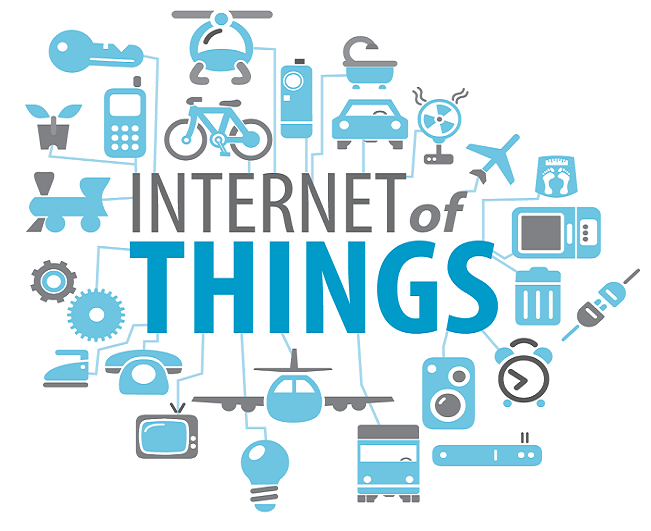
\includegraphics[width=10cm]{images/IoT.png}
	\end{center}
	\caption{Internet of Things *http://www.pcworldenespanol.com/}
	\label{fig:IoT}
\end{figure}

\section{Obxeto}

O obxetivo principal deste proxecto vai ser o de realizar a monitorización de un procesado de un pedido ou picking nun almacén para un operario a través dun terminal de operador inalambrico.

\begin{figure}[H]
	\begin{center}
		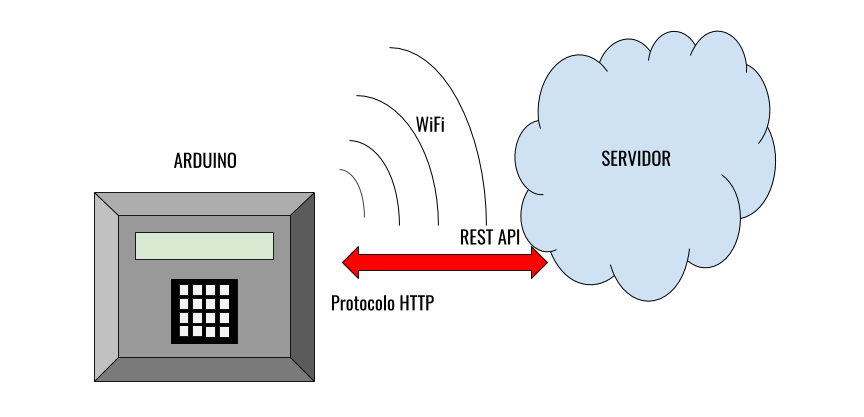
\includegraphics[width=10cm]{images/esquema_xeral.png}
	\end{center}
	\caption{Esquema xeral do proxecto}
	\label{fig:IoT}
\end{figure}

Debido ós altos costes dos terminales, como por exemplo SYMBOL VC5090, pensouse en realizalo cunha placa Arduino e o módulo WiFi ESP8266 pola súa capacidade de programación e, por suposto, polo seu precio.
Por outro lado, tamén conta cunha interfaz web para o almacén, podendo gestionar tanto os productos coma os pedidos.

\begin{figure}[H]
	\begin{center}
		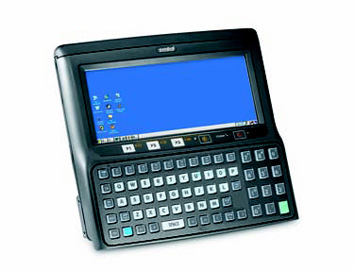
\includegraphics[width=10cm]{images/symbol_VC5090.jpg}
	\end{center}
	\caption{Terminal de operador SYMBOL VC5090 *http://www.datanet.com.au/}
	\label{fig:IoT}
\end{figure}

Para elo, vaise dividir o documento \textbf{Memoria} en requerimentos hardware, onde se vai detallar os compoñentes hardware usados, e requerimentos software, onde se explicará a parte de programación da parte de \txtbf{Arduino} e a parte de \textbf{Django RESTful Service}.

\chapter{Conceptos previos}

\section{Preparación de pedidos ou picking}

No mundo da loxística, realizar picking de un producto consiste en ir a unha estantería ou zona concreta dentro do almacén para recoller os productos requeridos para un pedido. É un proceso importante dentro empresas tanto pequenas coma grades, polo que é importante a súa optimización e mecanización.

\subsection{Formas de preparación de pedido}
Dentro picking, existen infinitas metodoloxías tradicionais de xestionalo, que veñen determinadas pola tipoloxía do almacén, niveis de servicios que da a empresa, etc. 
Pódense clasificar segundo:

\begin{itemize}
    \item Onde o efectuamos
        \begin{itemize}
            \item \textbf{De home a pedido:} Os operarios recorren o almacén e seleccionar o producto. 
            \item \textbf{De producto a home:} O producto é o que se desplaza ata o posto no que está o operario. Ten unha maior inversión económica pero reduce o tempo.
        \end{itemize}
    \item Como extraemos a mercancía
        \begin{itemize}
            \item \textbf{Pedido a pedido: } Os operarios preparan de forma individual os pedidos, é decir, solo preparan un pedido á vez. 
            \item \textbf{Por oleaxe: } Realizan picking de varios pedidos á vez. Merece a pena se hai poucos pedidos e moita repetividade. 
        \end{itemize}
    \item A unidade de extracción
        \begin{itemize}
            \item \textbf{De caixas completas.}
            \item \textbf{De unidades soltas.}
        \end{itemize}
\end{itemize}

En concreto neste proxecto, a metodoloxía vai ser picking de home a producto, de pedido a pedido e de unidades soltas.

\section{Arduino}
\subsection{Historia}

Arduino nace polo ano 2005 como un proxecto de estudiantes no Instituto de Diseño Interactivo Ivrea de Italia (IDII), onde os alumnos experimentaban con distintos tipos de microcontroladores. A idea era crear unha ferramenta moderna, sencilla, barata e fácil de usar. Foi así como empezaron a desenvolvela baixo a licencia de Open Source, para que todo o mundo poidese contribuir explotando por todo o mundo.

\subsection{Placas}

Hai moitas variedades de placas. Na táboa de abaixo móstranse as características das principais:

\begin{table}[htb]
\begin{center}
\resizebox{16cm}{!} {
\begin{tabular}{|c|m{3cm}|m{3.5cm}|m{2cm}|m{2cm}|m{2cm}|m{2cm}|m{2cm}|m{2cm}|c|c|}
\hline
Nombre & Procesador & Operating/Voltage Input & CPU Speed & Analogic In/Out & Digital IO/PWM & EEPROM & SRAM & FLASH & USB & UART \\
\hline
101 & Intel Curie & 3.3V/7-12V & 32MHz & 6/0 & 14/4 & - & 24 & 196 & Regular & - \\ 
\hline
Gemma & ATtiny85 & 3.3 V / 4-16 V & 8 MHz & 1/0 & 3/2 & 0.5 & 0.5 & 8 & Micro & 0 \\
\hline
LilyPad & ATmega168V \newline ATmega328P & 2.7-5.5 V/2.7-5.5 V & 8MHz & 6/0 & 14/6 & 0.512 & 1 & 16 & - & - \\
\hline
LilyPad SimpleSnap & ATmega328P & 2.7-5.5 V/2.7-5.5 V & 8 MHz & 4/0 & 9/4 & 1 & 2 & 32 & - & - \\
\hline
LilyPad USB & ATmega32U4 & 3.3 V/3.8-5 V & 8 MHz & 4/0 & 9/4 & 1 & 2.5 & 32 & Micro & - \\
\hline
Mega 2560 & ATmega2560 & 5V/7-12 V & 16 MHz & 16/0 & 54/15 & 4 & 8 & 256 & Regular & 4 \\
\hline
Micro & ATmega32U4 & 5 V/7-12 V & 16 MHz & 12/0 & 20/7 & 1 & 2.5 & 32 & Micro & 1 \\
\hline
MKR1000 & SAMD21 Cortex-M0+ & 3.3 V/ 5V  & 48MHz  & 7/1 & 8/4 & - & 32 & 256 & Micro & 1 \\
\hline
Pro & ATmega168 ATmega328P & 3.3 V/3.35-12 V \newline  5 V/5-12 V & 8 MHz  \newline  16 MHz & 6/0 & 14/6 & 0.512 \newline 1 & 1   2 & 16  32 & - & 1 \\
\hline
Pro Mini & ATmega328P & 3.3 V / 3.35-12 V \newline  5 V / 5-12 V & 8 MHz \newline  16 MHz & 6/0 & 14/6 & 1 & 2 & 32 & - & 1 \\
\hline
Uno & ATmega328P & 5 V / 7-12 V & 16 MHz & 6/0 & 14/6 & 1 & 2 & 32 & Regular & 1 \\
\hline
Zero & ATSAMD21G18 & 3.3 V / 7-12 V & 48 MHz & 6/1 & 14/10 & - & 32 & 256 & 2 Micro & 2 \\
\hline
Due & ATSAM3X8E & 3.3 V / 7-12 V & 84 MHz & 12/2 & 54/12 & - & 96 & 512 & 2 Micro & 4\\
\hline
Esplora & ATmega32U4 & 5 V / 7-12 V & 16 MHz & - & - & 1 & 2.5 & 32 & Micro & - \\
\hline
Ethernet & ATmega328P & 5 V / 7-12 V & 16 MHz & 6/0 & 14/4 & 1 & 2 & 32 & Regular & - \\
\hline
Leonardo & ATmega32U4 & 5 V / 7-12 V & 16 MHz & 12/0 & 20/7 & 1 & 2.5 & 32 & Micro & 1 \\
\hline
Mega ADK & ATmega2560 & 5 V / 7-12 V & 16 MHz & 16/0 & 54/15 & 4 & 8 & 256 & Regular & 4 \\
\hline
Mini & ATmega328P & 5 V / 7-9 V & 16 MHz & 8/0 & 14/6 & 1 & 2 & 32 & - & - \\
\hline
Nano & ATmega168 \newline ATmega328P & 5 V / 7-9 V & 16 MHz & 8/0 & 14/6 & 0.512  1 & 1  2 & 16 32 & Mini & 1 \\
\hline
Yún & ATmega32U4 \newline AR9331 Linux & 5 V & 16 MHz \newline 400MHz & 12/0 & 20/7 & 1 & 2.5 \newline  16MB & 32 \newline   64MB & Micro & 1 \\
\hline
Arduino Robot & ATmega32u4 & 5 V & 16 MHz & 6/0 & 20/6 & 1 KB (ATmega32u4)/512 Kbit (I2C) & 2.5 KB (ATmega32u4) & 32 KB (ATmega32u4) of which 4 KB used by bootloader & 1 & 1 \\
\hline
MKRZero & SAMD21 \newline  Cortex-M0+32bit low power \newline ARM MCU & 3.3 V & 48 MHz & 7 (ADC 8/10/12 bit)/1 (DAC 10 bit) & 22/12 & No & 32 KB & 256 KB & 1 & 1 \\
\hline
\end{tabular}
}
\caption{Comparación de placas Arduino}
\label{taboa:comparacionPlacasArduino}
\end{center}
\end{table}

Neste proxecto vaise usar Arduino Mega 2560.

\subsection{Entorno de Programación}

O entorno de desenvolvemento integrado (Integrated Development Environment ou IDE) é un programa informático composto por un conxunto de ferramentas de programación. 

Arduino ten un IDE propio chamado Arduino IDE, pero por comodidade vaise empregar Atom con un plugin chamado \textit{PlatformIO}, que nos vai permitir poder compilar, subir e debbugear código na placa.

\begin{figure}[H]
	\begin{center}
		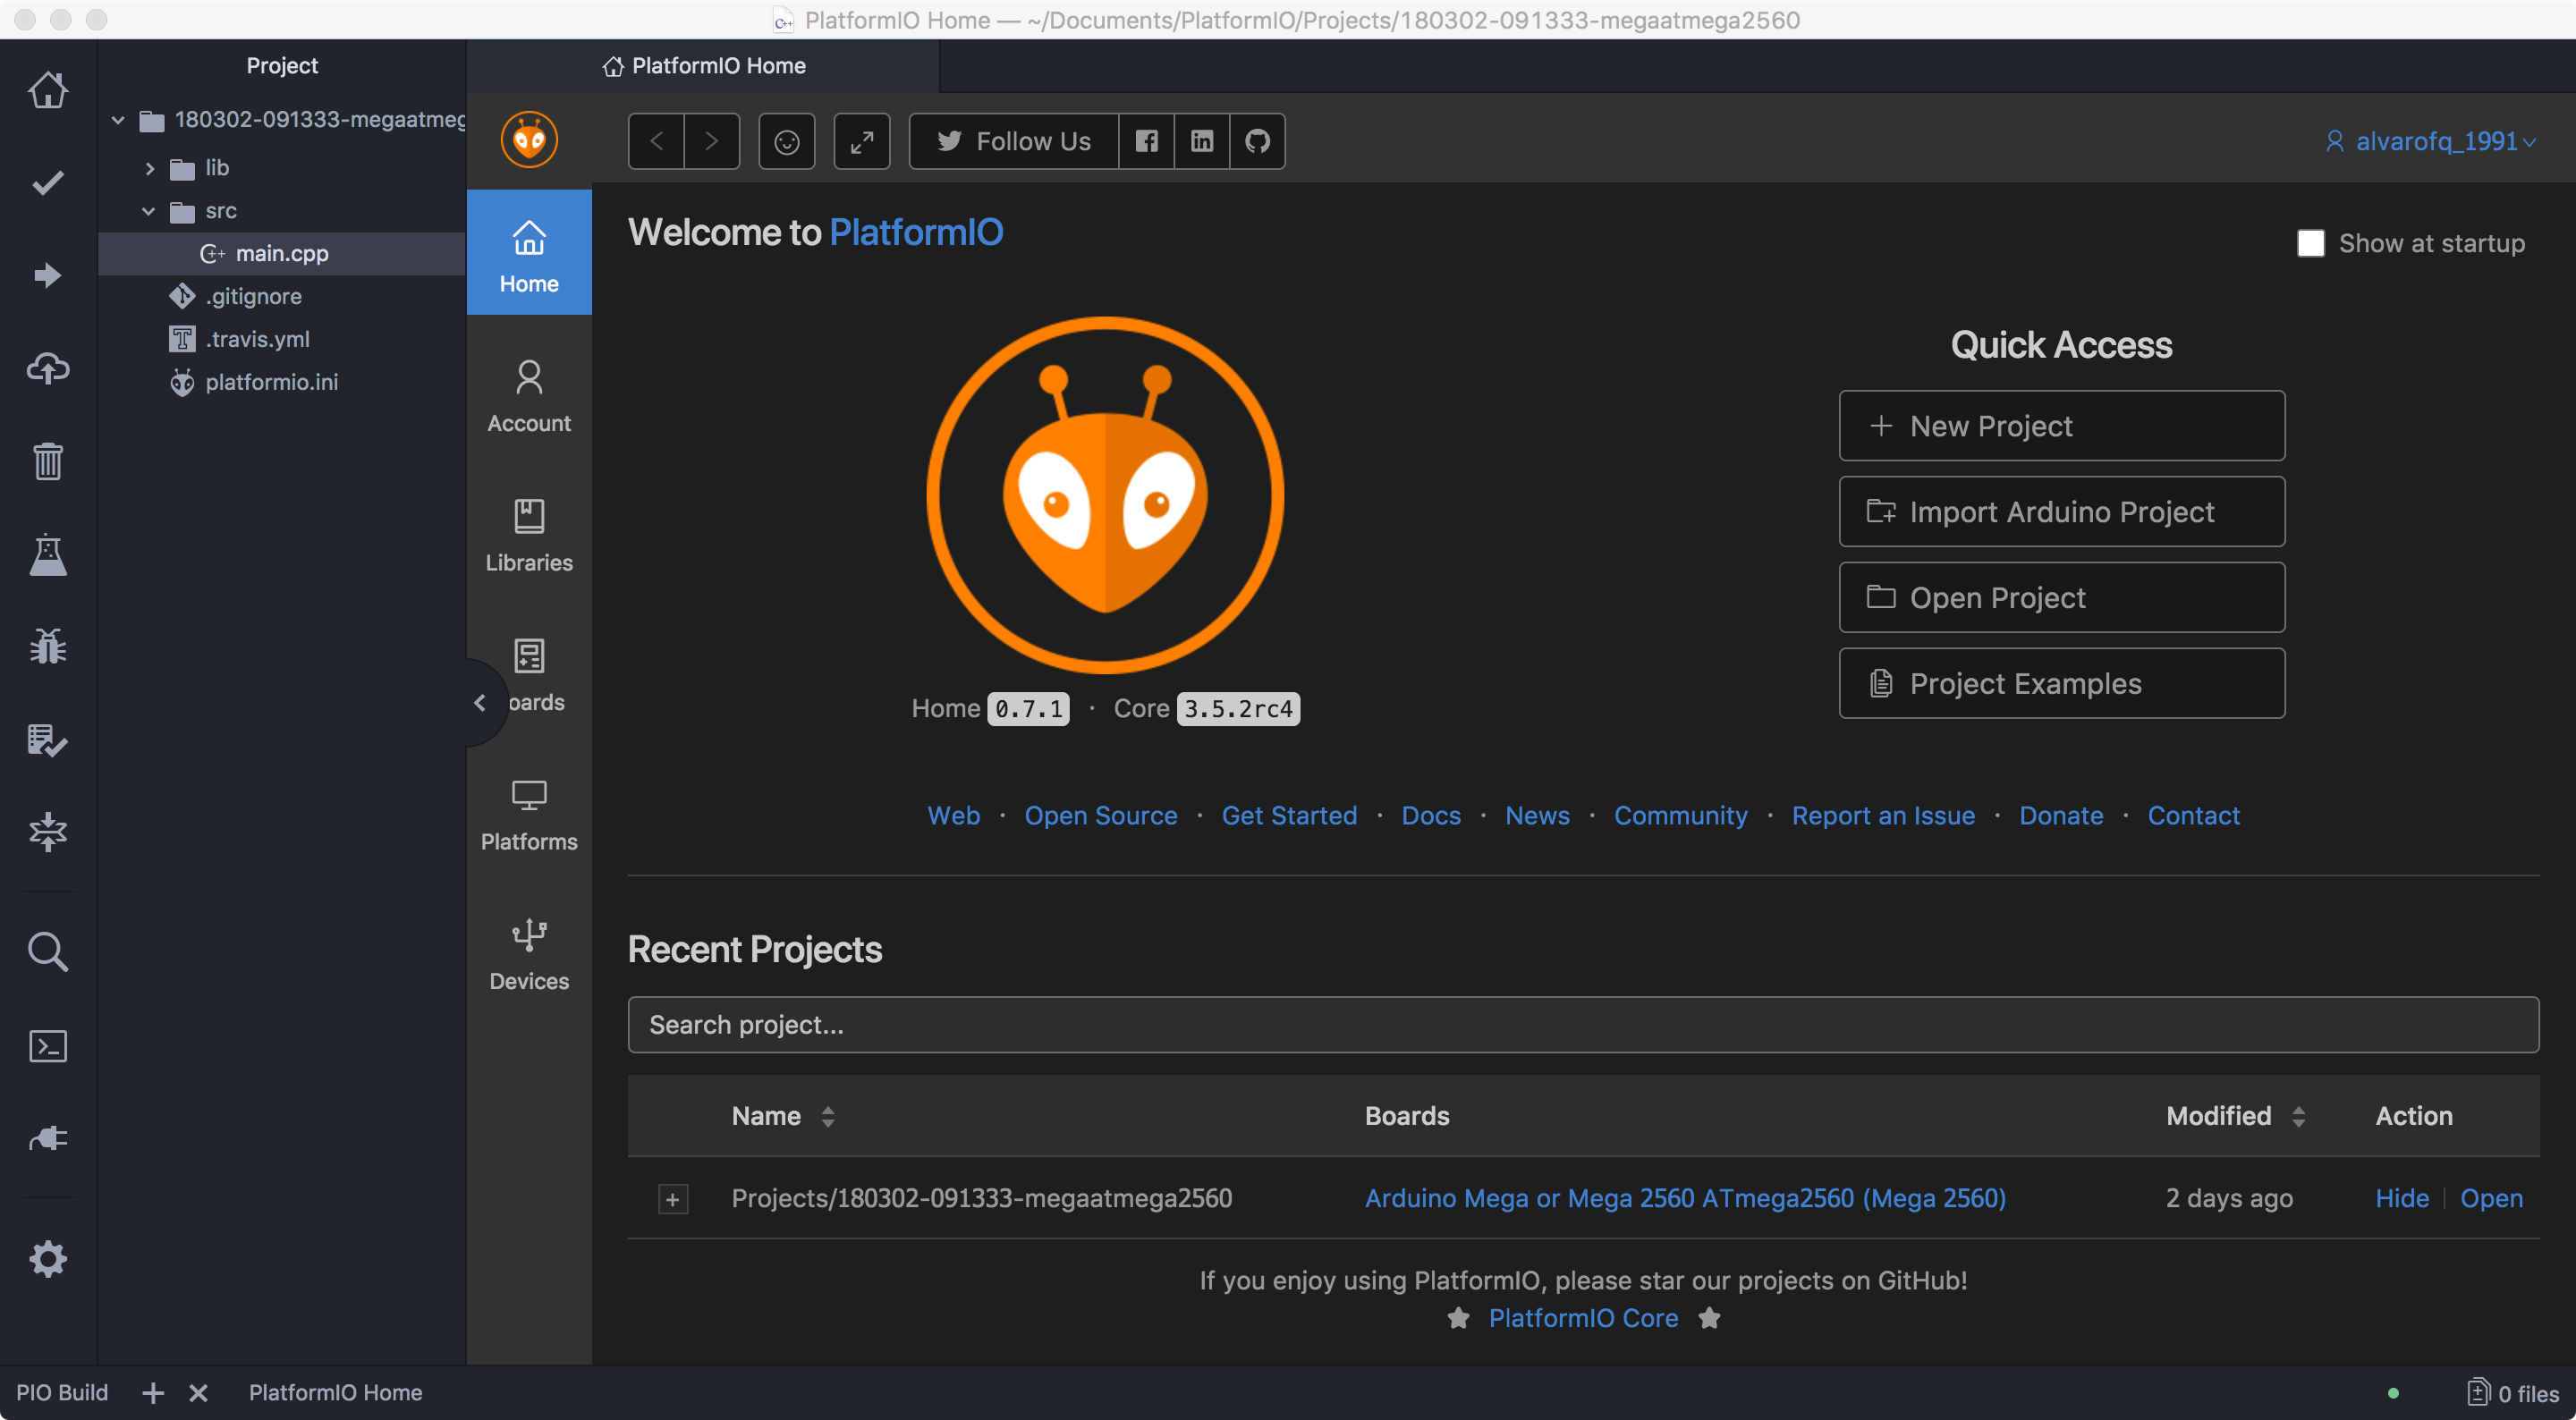
\includegraphics[width=15cm]{images/Atom.png}
	\end{center}
	\caption{Atom}
	\label{fig:Atom}
\end{figure}

Para a creación dun novo proxecto, faise click en New Project, poñéndolle un nome e seleccionando a placa usada, que neste caso vai ser Arduino Mega 2560.

\begin{figure}[H]
	\begin{center}
		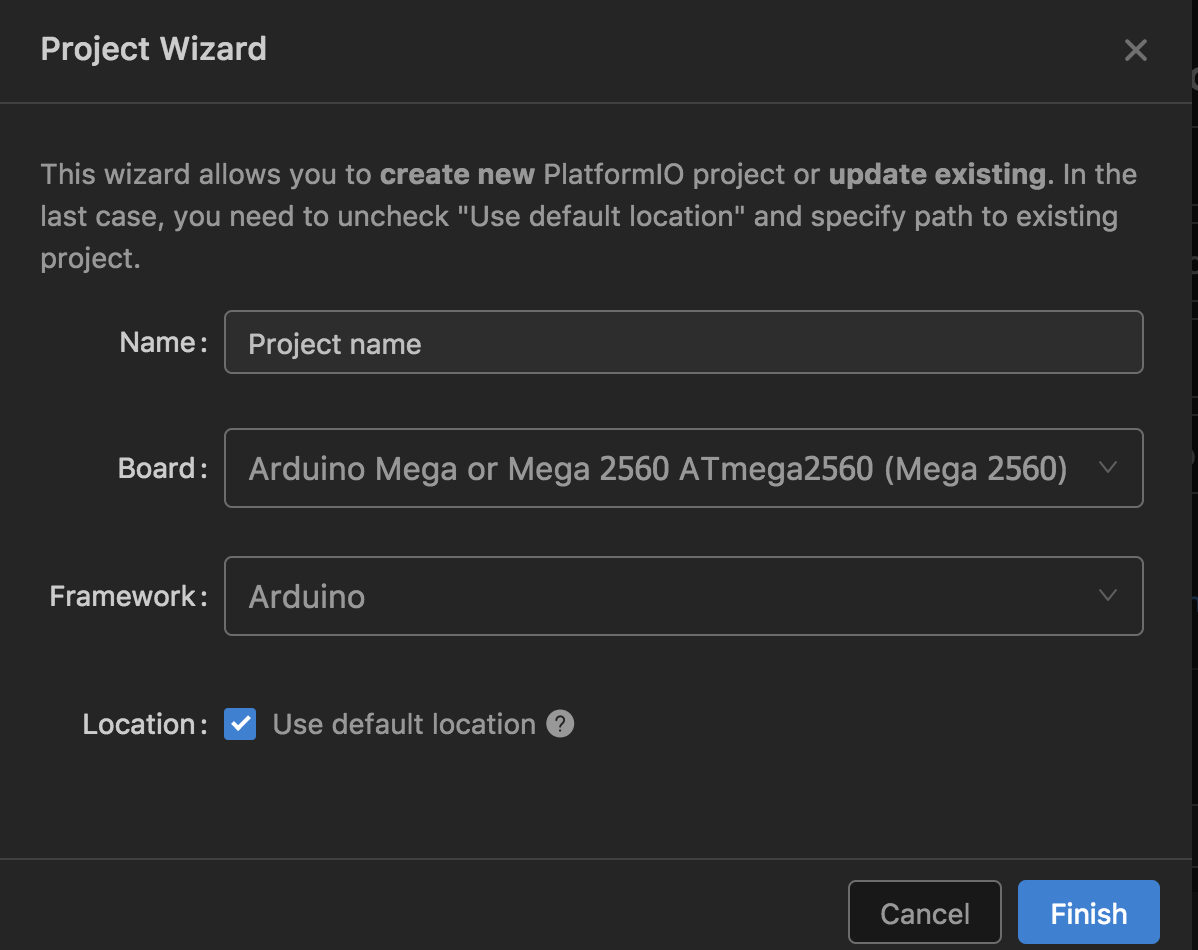
\includegraphics[width=8cm]{images/NewProject.png}
	\end{center}
	\caption{Novo Proxecto}
	\label{fig:NewProject}
\end{figure}

\subsection{Sketches}

Os programas de Arduino, tamén chamados Sketch, están compostos por un solo ficheiro con extensión \"{.ino"}, pero neste caso, o arquivo vai ter extensión \"{.cpp} como no lenguaxe de programación C++.

\subsection{Librerías}

Na nosa aplicación, podemos incorporar  librerías codificadas por outros programadores. Esto facilita á hora de programar e permite a abstracción facendo que o noso programa sexa moito máis fácil de elaborar e entender.

Disponse de infinidade de librerías para facilitar traballo, sendo todas elas Open Source.

Normalmente veñen comprimidas nun archivo ZIP e conteñen:
\begin{itemize}
\item Un archivo .cpp (código C++)
\item Un arquivo de declaracións con extensión .h que contén a declaración dunha ou varias clases.
\item Un directorio con varios exemplos para axudarnos a entendela.
\end{itemize}

Para incluir librerías no noso proxecto, na carpeta chamada "lib" importaranse, creando un packete para cada unha.

\begin{figure}[H]
	\begin{center}
		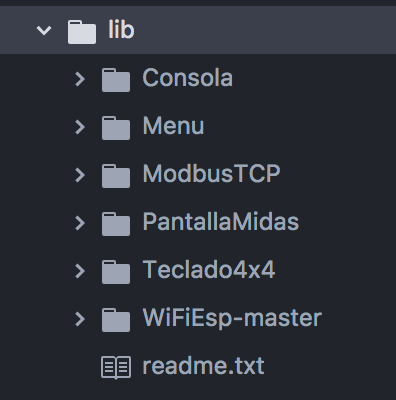
\includegraphics[width=7cm]{images/librerias.png}
	\end{center}
	\caption{Incluir librerías}
	\label{fig:LibreriasAtom}
\end{figure}

\subsection{Serial Monitor}

O plugin PlataformIO ten tamén a opción mostrar o que se comunique ca placa Arduino por medio do porto Serial.
Esto vai ser útil á hora do desenvolvemento xa que nos permite imprimir por pantalla datos ou estadísticas.
 Para eso iremos o apartado Serial Monitor e configuraremos o porto no que temos conectada a placa e os baudios:

\section{API REST}

API (Application Programming Incerface) é unha colección de funcións e métodos desenvolvidas para que outros usuarios poidan usalas. 
REST (Representatioal State Transfer) é unha arquitectura de desarrollo web que usa o estándar HTTP. 
Con API REST vai permitir o uso de unha función ou método que pertence a unha plataforma para o uso.

\subsection{Arquitectura}

\subsubsection{Identificación de recursos con URI's}

Un recurso representa unha sección, arquivo ou contido que queremos obter ou modificar. Para poder identificalo, usaremos URI's, que teñen que cumprir:
\begin{itemize}
    \item Os nomes non poden levar verbos.
    \item Deben ser únicas.
    \item Non deben tomar en conta o formato.
    \item Deben ter unha xerarquía lóxica.
    \item Os filtrados de información faranse mediante parámetros HTTP.
    \item Debe usarse a súa forma plural.
\end{itemize}

\subsubsection{Métodos HTTP}

Os principais métodos son:

\begin{itemize}
    \item GET: Consulta e lectura de recursos.
    \item POST: Creación de recursos.
    \item PUT: Edición de recursos.
    \item DELETE: Eliminación de recursos.
    \item PATCH: Edicion de partes de recursos.
\end{itemize}

\chapter{Compoñentes Hardware}
\section{Arduino Mega 2560}

O Arduino Mega 2560 é un microcontralador basado no ATmega2560. Ten 54 pins de entrada/saída dixitais (dos cales 15 pódense empregar como saídas PWM), 16 entradas analóxicas, 4 UART (portas de serie de hardware), un oscilador de cristal de 16 MHz, unha conexión USB, unha toma de enerxía, un encabezado ICSP, e un botón de reset. Contén todo o necesario para soportar o desenvolvimento de aplicacións para este microcontrolador; simplemente conéctase a unha computadora con un cable USB ou aliméntase cun adaptador AC-to-DC ou batería para comezar. 

\begin{figure}[H]
	\begin{center}
		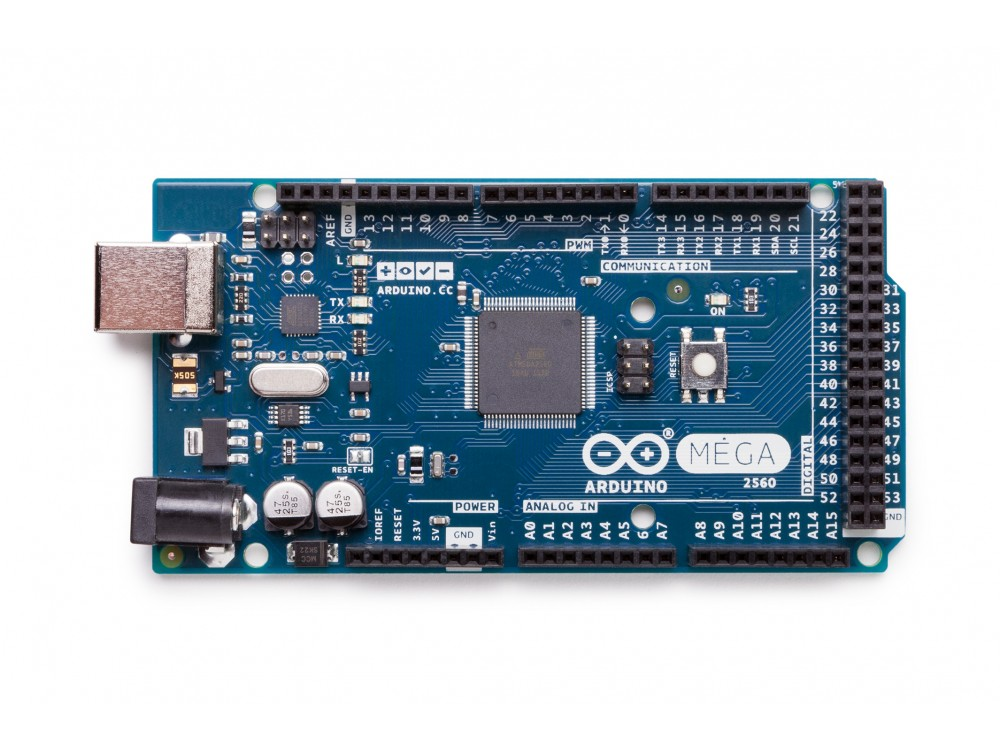
\includegraphics[width=7cm]{images/arduino_mega.jpg}
	\end{center}
	\caption{Arduino Mega 2560 *http://arduino.cc}
	\label{fig:ArduinoMega}
\end{figure}

\subsection{Alimentación eléctrica}

Pode ser alimentado a través da conexión USB ou cunha fonte de alimentación externa. A fonte de enerxía está seleccionada automaticamente. 

A placa pode funcionar nunha fonte externa de 6 a 20 voltios. Se se fornece con menos de 7V, con todo, o pin de 5V pode fornecer menos de 5V e pode volverse inestable. Se usa máis de 12V, o regulador de voltaxe pode sobrecalentarse e dañala. O rango recomendado é de 7 a 12V.

Os pines de alimentación son os seguintes:

\begin{itemize}
\item \textbf{Vin.} A tensión de entrada á placa cando está a usar unha fonte de enerxía externa (a diferenza de 5 voltios da conexión USB ou outra fonte de alimentación regulada). Pode fornecer a tensión a través deste pin ou, se fornecer a tensión a través do conector de enerxía, accédese a través deste pin.
\item \textbf{5V.} Este pin outorga un regulador de 5V desde o regulador do taboleiro. O taboleiro pode ser subministrado con enerxía desde a toma de alimentación de CC (7-12V), o conector USB (5V) ou a pin VIN do taboleiro (7-12V). A subministración de tensión a través dos pines de 5V ou 3.3V evita o regulador e pode danar a táboa. Non o aconsellamos.
\item \textbf{3V3.} Unha fonte de 3,3 voltios xerada polo regulador de a bordo. O sorteo máximo actual é de 50 mA.
\item \textbf{GND.} Pins de terra.
\item \textbf{IOREF.} Este pin proporciona a referencia de tensión coa que funciona o microcontrolador. Un escudo configurado correctamente pode ler a tensión de tecto IOREF e seleccionar a fonte de enerxía adecuada ou habilitar traductores de tensión nas saídas para traballar cos 5V ou 3.3V.
\end{itemize}

\section{Módulos ou periféricos}

\subsection{Pantalla LCD}

Para visualizar os pedidos dos operarios e xestionalos, empregarase unha pantalla LCD da marca Midas que ten unha resolución de 4 liñas x 40 caracteres. 

\begin{figure}[H]
	\begin{center}
		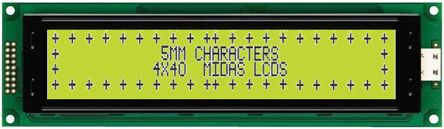
\includegraphics[width=8cm]{images/lcd.jpg}
	\end{center}
	\caption{Pantalla LCD Midas 4x40}
	\label{fig:PantallaLCD}
\end{figure}

A conexión da pantalla coa placa Arduino Mega vai ser da seguinte maneira:

\begin{figure}[H]
	\begin{center}
		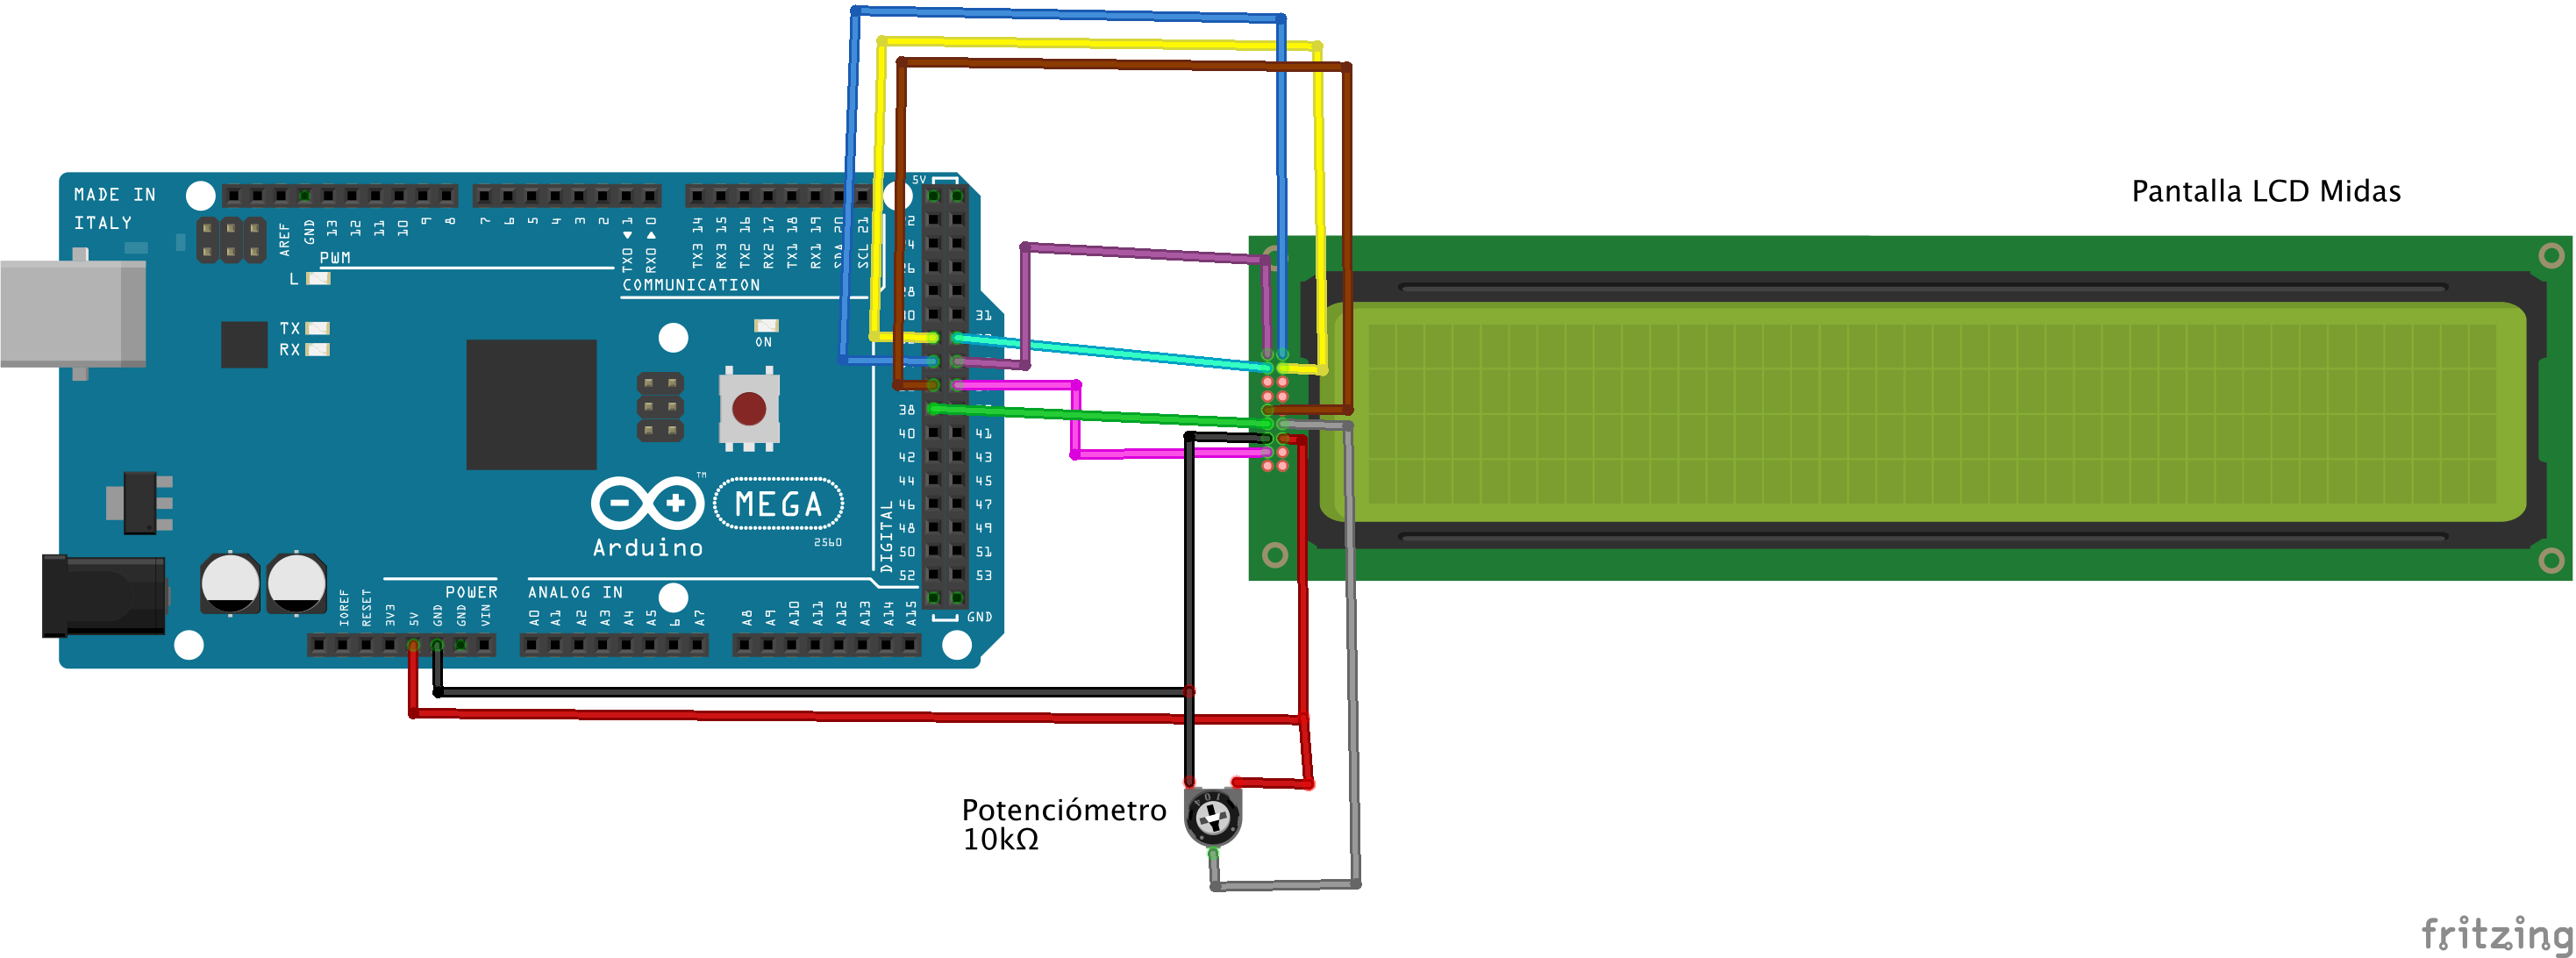
\includegraphics[width=15cm]{images/conexionArduinoLCD.png}
	\end{center}
	\caption{Conexión placa Arduino Mega con pantalla LCD Midas}
	\label{fig:ConexionPantalla}
\end{figure}

\begin{table}[h]
\begin{center}
\begin{tabular}{|c|c|c|}
\hline
Arduino & Pantalla Midas & Color \\
\hline
32 & DB4 & Amarelo \\
\hline
33 & DB5 & Cian\\
\hline
34 & DB6 & Azul \\
\hline
35 & DB7 & Morado \\
\hline
36 & E1 & Marrón \\
\hline
37 & E2 & Rosa \\
\hline
38 & RS & Verde \\
\hline
5V & Vdd & Vermello \\
\hline
GND & Vss & Negro \\
\hline
\end{tabular}
\caption{Conexión pines entre Arduino e Pantalla LCD Midas}
\label{TablaArduinoPantalla}
\end{center}
\end{table}

Para o control de alimentación, e, polo tanto, para o control de brillo da pantalla, vaise añadir un potenciómetro de 10k que ten o esquema reflexado na figura \ref{fig:ConexionPantalla} e os seguintes pines:

\begin{table}[htbt]
\begin{center}
\begin{tabular}{|c|c|c|}
\hline
Potenciómetro & Pantalla Midas & Arduino\\
\hline
IN & Vdd & 5V \\
\hline
OUT & V0 & -\\
\hline
\end{tabular}
\caption{Conexión do potenciómetro}
\label{TablaPotenciometro}
\end{center}
\end{table}

\subsection{Teclado Matricial}

Para poder indicarlle ó terminal que se completou unha caixa, vaise usar un teclado matricial 4x4.

\begin{figure}[H]
	\begin{center}
		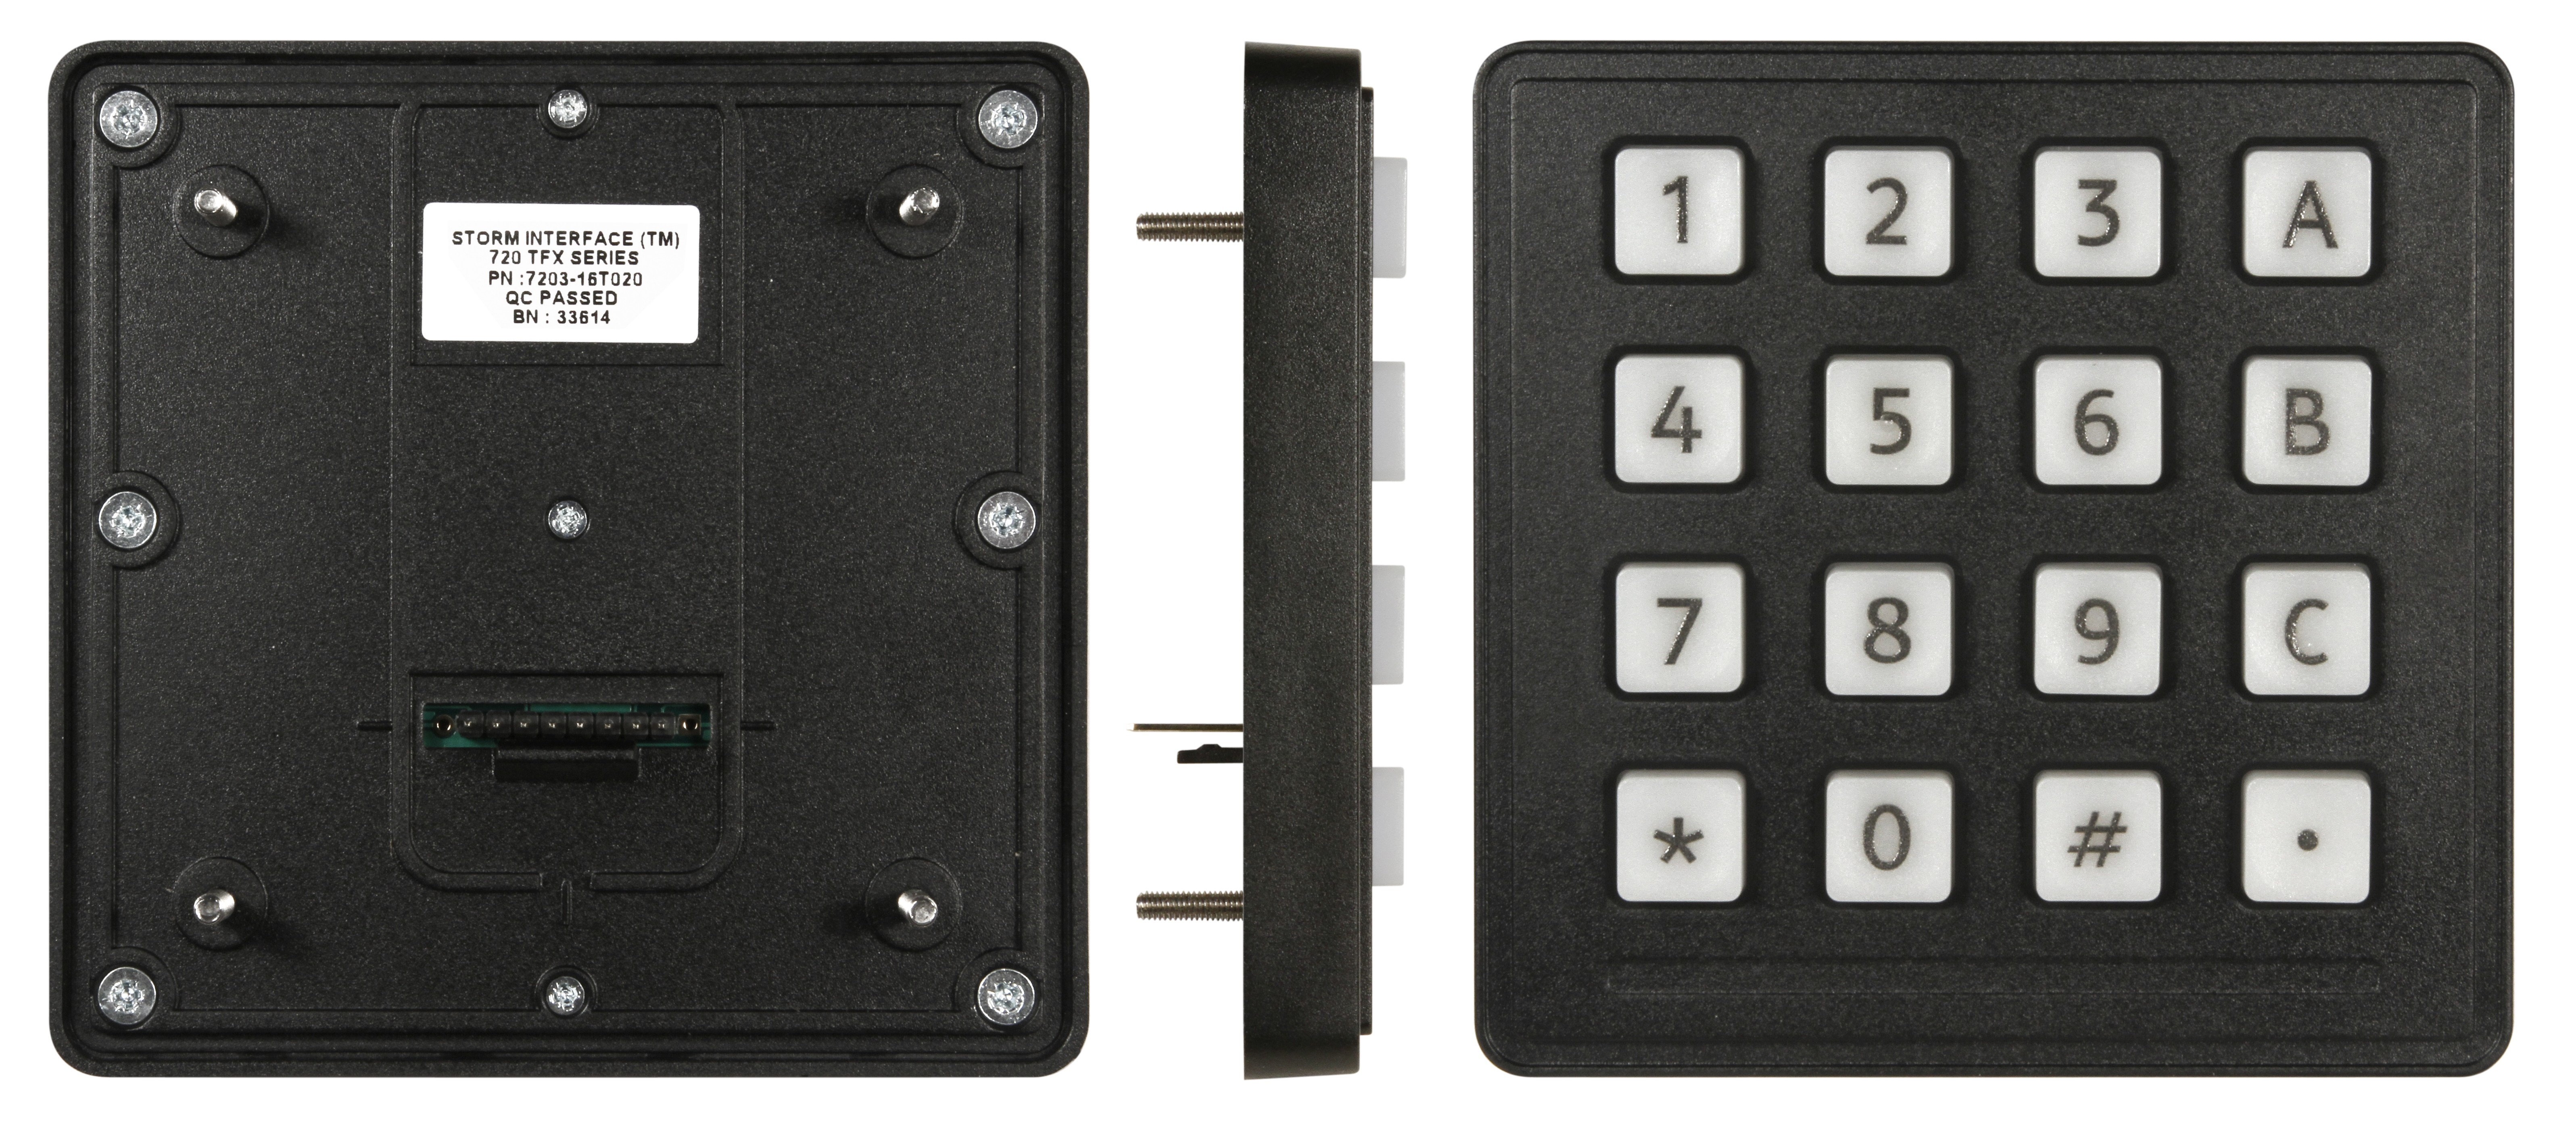
\includegraphics[width=8cm]{images/teclado_storm.jpg}
	\end{center}
	\caption{STORM 720TFX SERIES *http://www.storm-interface.com/storm-720tfx-series-16-button.html}
	\label{fig:TecladoStorm}
\end{figure}

A conexión con Arduino vai ser da seguinte maneira:

\begin{figure}[H]
	\begin{center}
		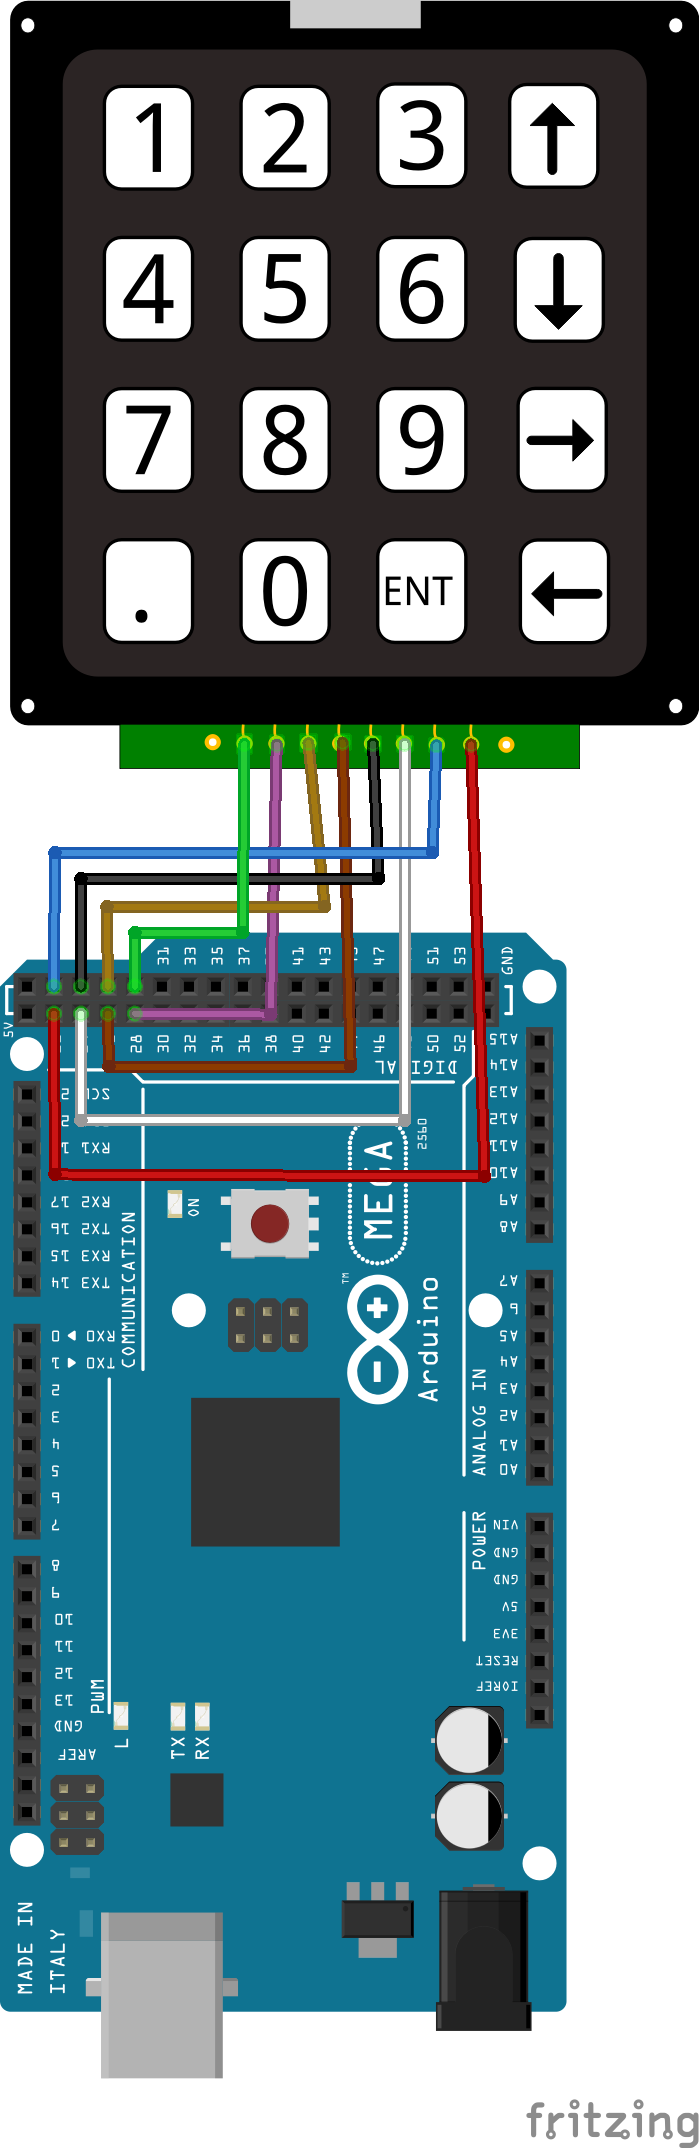
\includegraphics[scale=0.75]{images/conexionArduinoKeypad.png}
	\end{center}
	\caption{Conexión placa Arduino Mega con teclado 4x4 Matrix}
	\label{fig:ConexionESP8266}
\end{figure}

\begin{table}[H]
\begin{center}
\begin{tabular}{|c|c|c|}
\hline
Arduino & Keypad Storm & Color \\
\hline
22 & 01 & Vermello \\
\hline
23 & 02 & Azul\\
\hline
24 & 03 & Blanco \\
\hline
25 & 04 & Negro \\
\hline
26 & 05 & Marrón \\
\hline
27 & 06 & Ocre\\
\hline
28 & 07 & Verde \\
\hline
29 & 08 & Morado \\
\hline
\end{tabular}
\caption{Conexión pines entre Arduino e Teclado 4x4}
\label{TablaArduinoKeypad}
\end{center}
\end{table}

\subsection{ESP8266}

É un microprocesador de baixo custo con WiFi integrado fabricado por Espressif. Supuxo unha revolución á hora de conectar o Arduino a WiFi, xa que as placas existentes eran demasiado caras, como por exemplo WiFi Shield.

Ademáis, pode comportarse como un procesador completo, con moita máis potencia que a maioría das placas Arduino.

Existen moitos modelos de placas que integran o ESP8266; o módulo ESP01 é un dos primeiros en aparecer co chip ESP8266 e un dos módulos máis sinxelos e baratos.

\begin{figure}[H]
	\begin{center}
		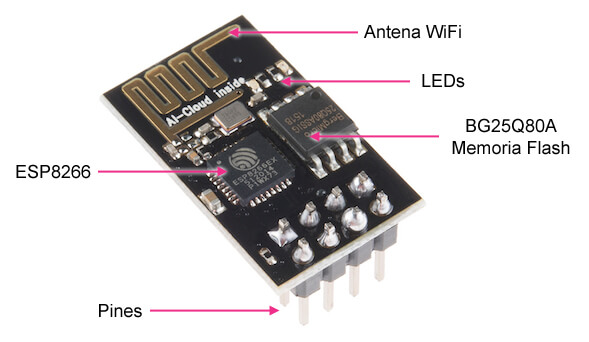
\includegraphics[width=12cm]{images/esp8266_conexion.jpg}
	\end{center}
	\caption{Esquema módulo ESP8266}
	\label{fig:EsquemaESP8266}
\end{figure}

En canto a comunicación WiFi, o ESP01 ten comunicación integrada 802.11  b/g/n, incluidos modos  Wi-Fi  Direct (P2P) e  soft-Ap. Inclúe unha pila de  TCP/IP completa, o que libera da maior parte do traballo de comunicación ó procesador.

\subsubsection{Esquema Eléctrico}

A conexión co módulo ESP8266 é bastante sinxela en comparación cos demáis compoñentes íntegros no proxecto. Ten os seguintes pines:

\begin{figure}[H]
	\begin{center}
		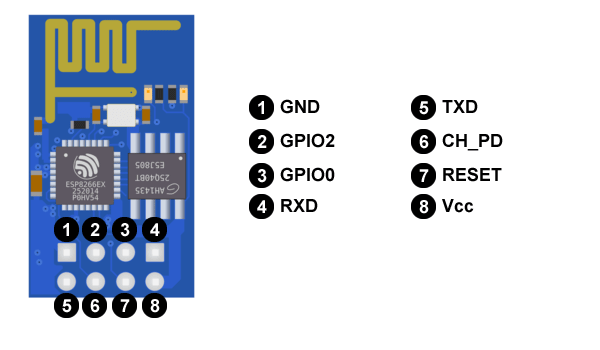
\includegraphics[width=10cm]{images/pines-esp01.png}
	\end{center}
	\caption{Pines módulo ESP8266}
	\label{fig:PinesESP8266}
\end{figure}

\begin{enumerate}
\item GND é a toma de terra.
\item GPIO2 é unha entrada/saida de propósito xeral. É o pin dixital número 2.
\item GPIO0 é unha entrada/saida de propósito xeral. É o pin dixital número 0.
\item RxD é o pin por onde se reciben os datos no porto serie. Pódese usar como pin dixital GPIO: sería o número 3.
\item TxD é o pin por onde se transmiten os datos no porto serie. Pódese usar como pin dixital GPIO: sería o número 1.
\item CH\_PD é o pin que o apaga ou encende: se está a 0V (LOW) apágase a 3,3V (HIGH), encéndese.
\item RESET é o pin que o resetea: se está a 0V (LOW) resetéase.
\item Vcc é por onde se alimenta. Funciona a 3,3 V.
\end{enumerate}

A única dificultade que imos ter vai ser á hora de alimentalo, xa que ten unha tensión de alimentación de 3,3V. En ningún caso pode alimentarse cunha tensión superior a 3,6 V, ou dañaríamolo.

Por outro lado, o consumo non pode sobrepasar o amperaxe de 200mA. O regulador do voltaxe de Arduino de 3,3V so pode proporcionar 50mA (150mA como máximo), polo que a alimentación é insuficiente e teríamos que alimentalo externamente para non sufrir cortes.

A comunicación mediante porto serie conectando os pines RxD e TxD.

A conexión coa placa vai ser a seguinte:

\begin{figure}[H]
	\begin{center}
		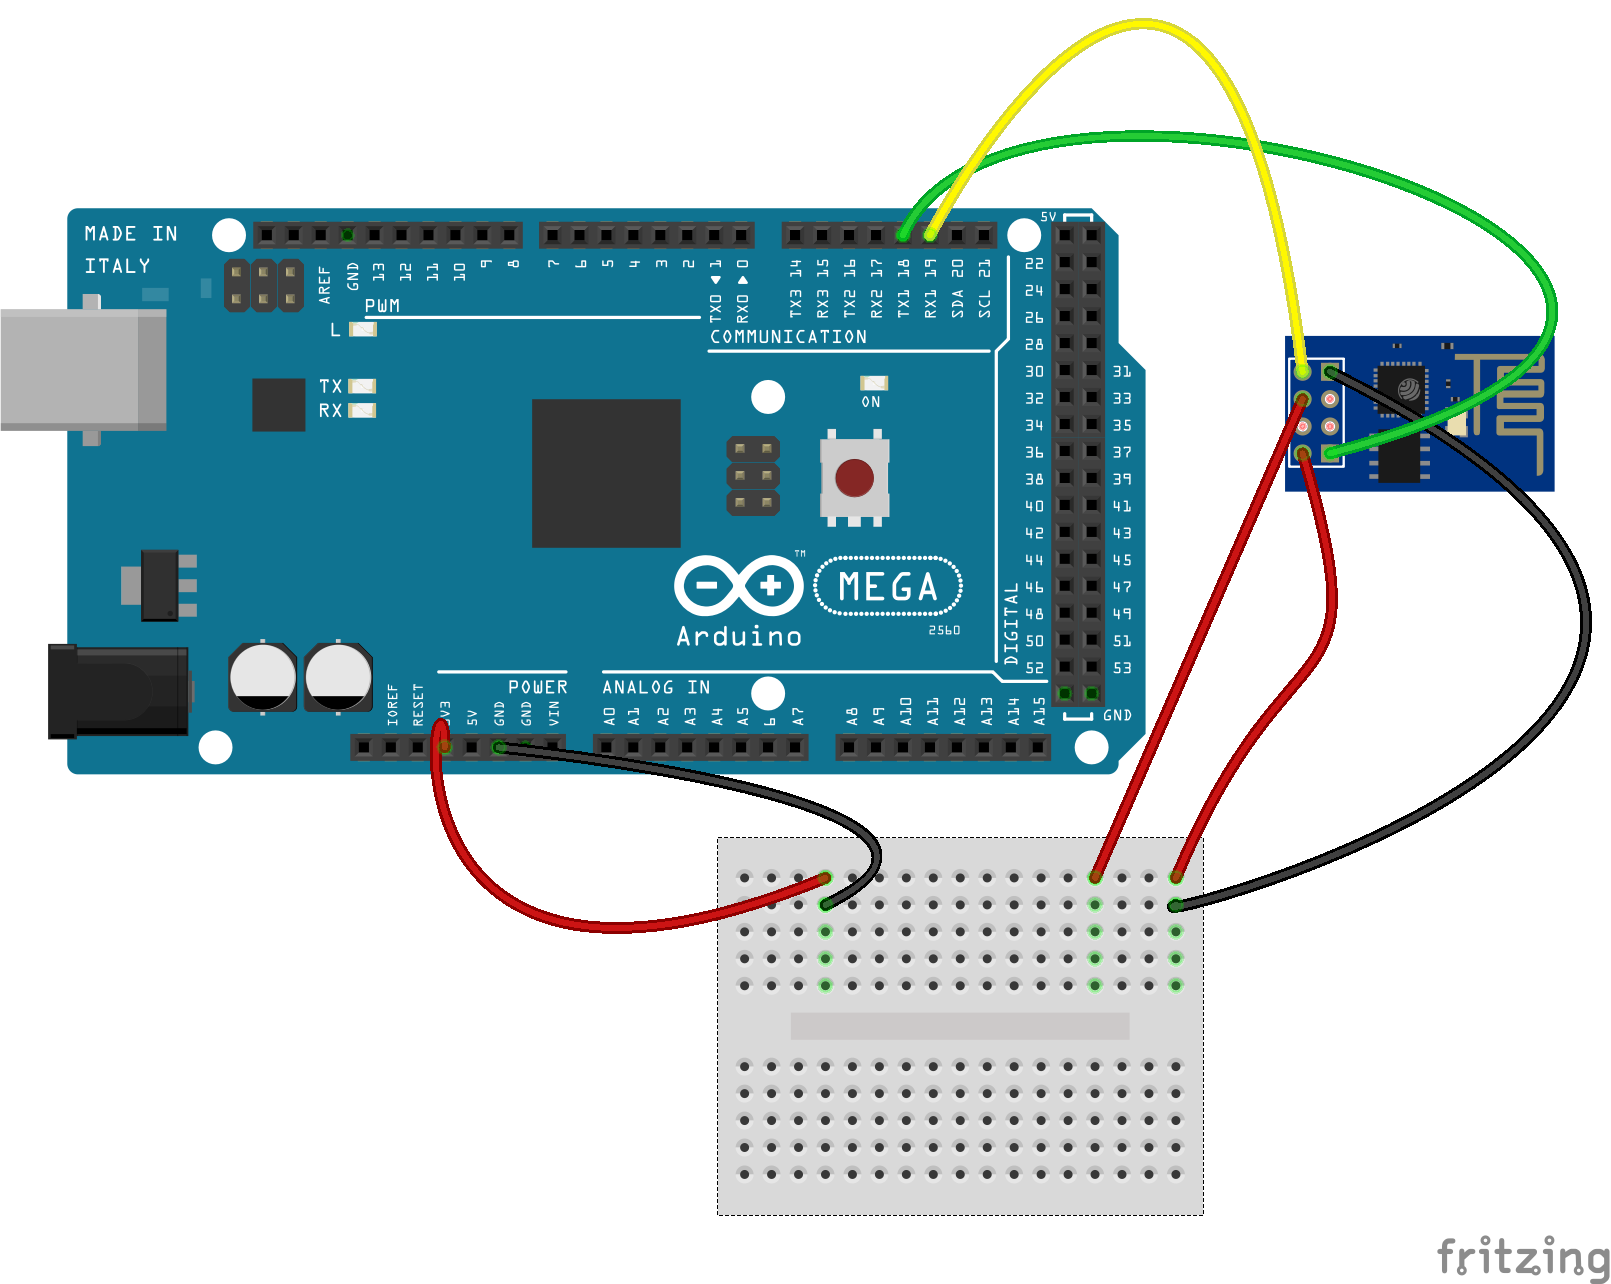
\includegraphics[width=10cm]{images/conexionArduinoESP8266_WiFiEsp.png}
	\end{center}
	\caption{Conexión placa Arduino Mega con módulo ESP8266}
	\label{fig:ConexionESP8266}
\end{figure}

\begin{table}[htbt]
\begin{center}
\begin{tabular}{|c|c|}
\hline
Arduino & ESP8266 \\
\hline
3,3V & Vcc \\
\hline
GND & GND \\
\hline
TX1(18) & RxD \\
\hline
Rx1(19) & TxD \\
\hline
3,3V & CH\_PD \\
\hline
\end{tabular}
\caption{Conexión pines entre Arduino e ESP8266}
\label{TablaArduinoESP8266_WiFiEsp}
\end{center}
\end{table}

\chapter{Compoñentes software}

Neste capítulo vaise dividir en dúas partes: a parte de programación do Arduino Mega 2560 e a parte da creación do servidor web con servicios API REST.

\section{Programa Arduino}

\subsection{Diagrama de fluxo}

\begin{figure}[H]
	\begin{center}
		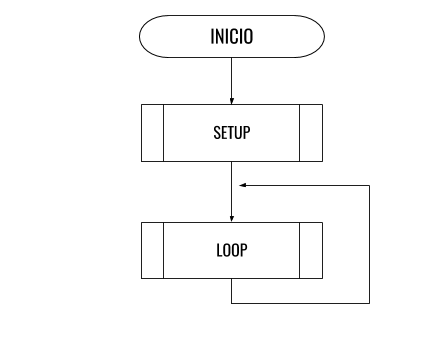
\includegraphics[width=5cm]{images/diagrama_flujo_inicio.png}
	\end{center}
	\caption{Diagrama de fluxo do programa principal Arduino}
	\label{fig:FluxoPrincipal}
\end{figure}

\begin{figure}[H]
	\begin{center}
		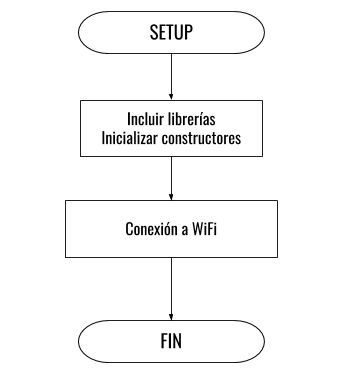
\includegraphics[width=6cm]{images/diagrama_flujo_setup.png}
	\end{center}
	\caption{Diagrama de fluxo de SETUP Arduino}
	\label{fig:FluxoSETUP}
\end{figure}

\begin{figure}[H]
	\begin{center}
		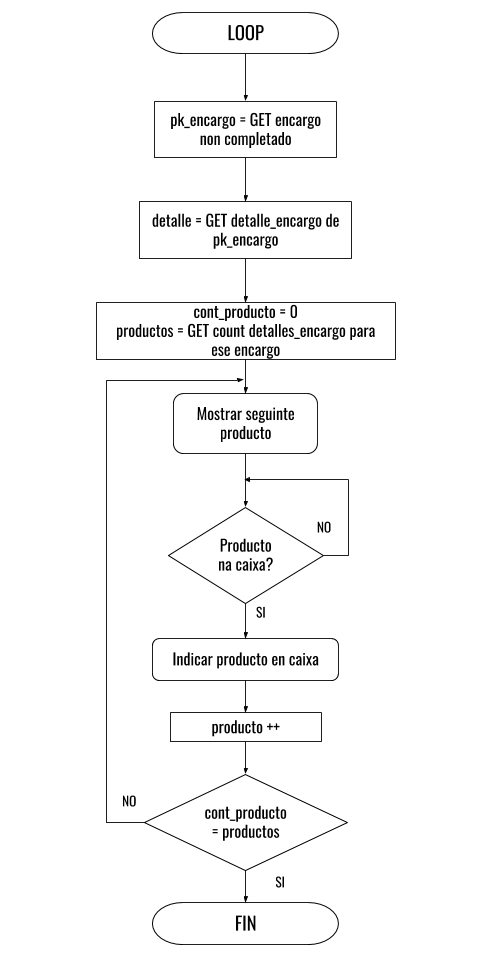
\includegraphics[width=8cm]{images/diagrama_flujo_loop.png}
	\end{center}
	\caption{Diagrama de fluxo de LOOP Arduino}
	\label{fig:FluxoLOOP}
\end{figure}
 
 \subsection{Pantalla LCD}

Vaise usar a librería \textit{PantallaMidas} para manexar a parte de programación da pantalla LCD. Esta librería inicialízase pasandolle por parámetros ó constructor os pines que está conectado. Faise da seguinte maneira:

\begin{minted}{cpp}
PantallaMidas pantalla(DB4, DB5, DB6, DB7, E1, E2, RS);
\end{minted}

Para inicializar a pantalla LCD, débese configurala. Neste caso vaise usar a configuración de bus de 4 bits e ten os seguintes pasos reflexados na Figura.

\begin{figure}[H]
	\begin{center}
		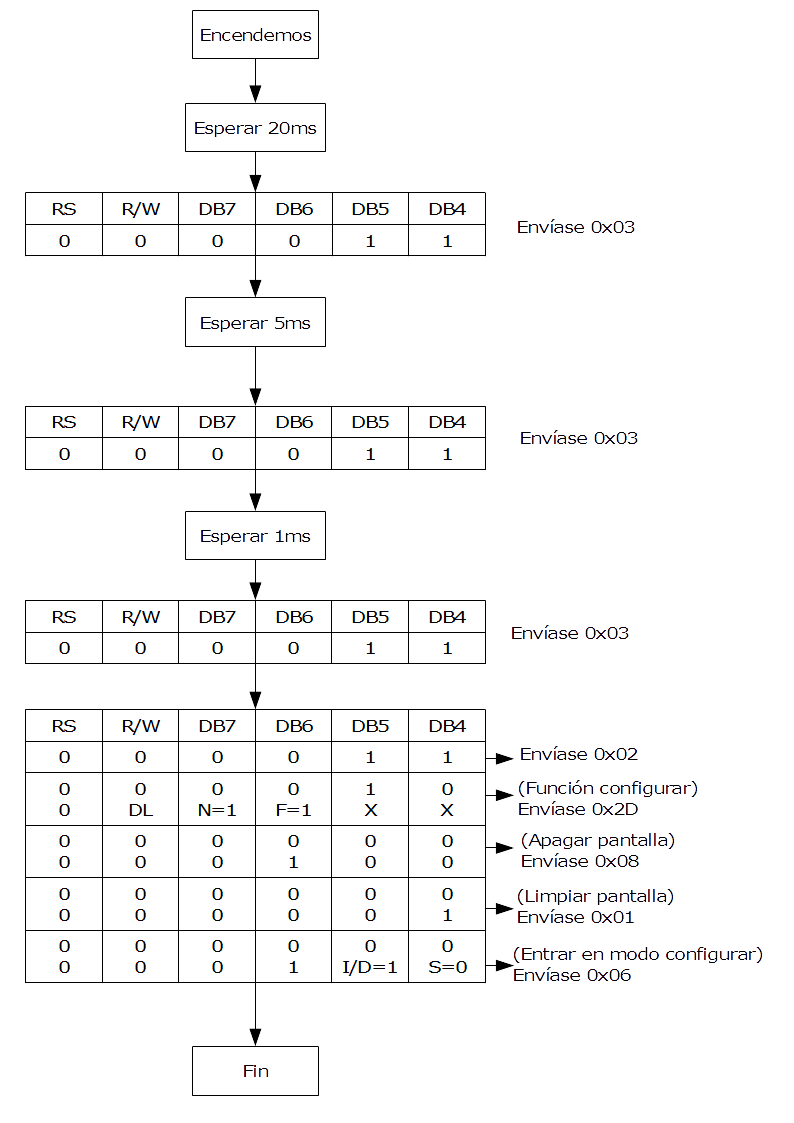
\includegraphics[scale=0.6]{images/inicializar_lcd.png}
	\end{center}
	\caption{Diagrama de Flujo iniciación pantalla LCD Midas}
	\label{fig:DiagramaFlujoPantalla}
\end{figure}

Para elo, usarase o metodo \textit{configura} como se mostra a continuación:
\begin{minted}{cpp}
pantalla.configura();
\end{minted}

\subsection{Teclado Matricial}

Para usar este compoñente, elaborouse unha clase en C++ que permite a identificación da tecla pulsada.

Para poder usar esta clase, hai que declarar un constructor pasandolle por referencia os pines e un String cos caracteres asociados. Un exemplo é o seguinte:

\begin{minted}{cpp}
Teclado4x4 teclado(F1, F2, F3, F4, C1, C2, C3, C4, caracteres);
\end{minted}

Unha vez feito o constructor, a función \textit{configura} vai configurar o teclado para poder manexalo.

\begin{minted}{cpp}
teclado.configura();
\end{minted}

Esta clase ten a función chamada \textit{comprueba()} que comproba se se pulsou unha determinada tecla devolvendo o caracter pulsado. Un exemplo:

\begin{minted}{cpp}
char caracter = teclado.comprueba();
\end{minted}


\subsection{ESP6288 ESP-01}

Os comandos básicos para a comunicación entre o módulo e a placa Arduino chámanse AT. O básicos reflexanse na seguinte táboa:

\begin{table}[!h]
\centering
\resizebox{16cm}{!} {
\begin{tabular}{|c|c|c|c|c|}
\hline
Comando & Descripción & Resposta & Configuración & Parámetros \\
\hline
AT & Test de inicio & OK & - & - \\
\hline
AT+RST & Restea o módulo & Module info & - & -\\
\hline
AT+GMR & Devolve a versión \newline do módulo & Fw Version & - & - \\
\hline
AT+CWMODE & Configura o  \newline modo WiFi & Mode set & AT+CWMODE=(Modo) & Modo 1=Sta, 2=AP, 3=both\\
\hline
AT+CWLAP & Lista todos os Puntos de Acceso (AP) & list of AP & - & - \\
\hline
AT+CWJAP & Conéctase a AP & OK & AT+CWJAP=(ssid),(pwd) & ssid= Nombre red de AP, pwd= contraseña de AP\\
\hline
AT+CWQAP & Finaliza a conexión con AP &  & AT+CWQAP & \\
\hline
AT+CWSAP & Configura os \newline parametros da AP & & AT+CWSAP=(ssid),(pwd), \newline (chl),(ecn) & ssid, contraseña, \newline canal, encriptacion \\
\hline
AT+CWLIF & Comproba a \newline conexión IP do módulo &  & AT+CWLIF &  \\
\hline
AT+CIPSTATUS & Comproba a conexión & (id),(tipo),(direccion),(porto) & AT+CIPSTATUS & -   \\
\hline
\end{tabular}
}
\caption{Comandos básicos AT}
\label{comandosAT}
\end{table}

Usaremos unha librería Open Source \textit{WiFiEsp} que nos facilitará a programación con comandos AT, xa que están implementados mediante funcións.

Pódese atopar manuais e exemplos no repositorio: textit{https://github.com/bportaluri/WiFiEsp}.

\section{Django RESTful Web Framework}

É unha librería que nos vai permitir construir un API REST sobre Django. Ofrece unha diversidade de métodos e funcións para a xestión dos recursos.

Esta librería é totalmente portable; podese usar tanto con Windows, Linux ou Mac OSX. Neste proxecto vaise usar o sistema operativo MacOs Hight Sierra.

A continuación móstrase como creala:

\subsection{Crear directorio base}

Vaise crear un directorio onde vai estar contido o código

\begin{minted}{bash}
  $ mkdir tfg_django
  $ cd tfg_django
\end{minted}

\subsection{Configurar entorno virtual}

Esto vainos permitir aislar as dependencias do proxecto, eliminando os conflictos de librerías locais do sistema.
\begin{minted}{bash}
  $ virtualenv tutorial
  $ source tfg_django/bin/activate #esto activará o noso entorno virtual.
\end{minted}

A continuación, instalaranse os paquetes necesarios.

\begin{minted}{bash}
  $ pip install django #instalar o paquete de django
  $ pip install djangorestframework #instalar o paquete de Django Rest Framework
\end{minted}

\subsection{Crear proxecto e configuración inicial}

Vaise crear o proxecto dentro do directorio base e inicializar a configuración. A API vaise chamar \textit{almacen} e vaise crear unha aplicación que se chamará \textit{encargos}.

\begin{minted}{bash}
  $ django-admin.py startproject almacen
  $ cd encargos
  $ django-admin.py startapp encargos
\end{minted}


\chapter{Resultados}




\chapter{Conclusións}

As melloras que se poden aplicar poden ser as seguintes:

\begin{itemize}
    \item Mellora da interfaz do servicio web
    \item Autentificación do operador mediante uso dun módulo que reconoza as huellas de actilares
\end{itemize}


\begin{thebibliography}{99}

\bibitem{IoT} \textsc{Brian Russell, Drew Van Duren}; \textit{Practical Internet of Things Security}, PACKT Publishing (Xuño 2016).
\bibitem{Django} \textsc{Gastón C. Hillar}, \emph{Building RESTful Python Web}, PACKT Publishing (Outubro 2016).
					
\end{thebibliography}

\stopcontents[parts]

\cleardoublepage
%%%%%%%%%%%%%%%%%%%%%%%%%%%%%%%%%%%%%%%%%%%%%%%%%%%%%%%%%%%%%%%%%%%%%%%%%%%%%%%%%%%%%%%%%%%%%%%%%%%%%%%%%%%%%%%%%%%%%%%%%%%%%%%%%%%%%%%%%%%%%%%%%%%%%%%%%%%%%%%%%%%%%%%%%%%%%
%%%%%%%%%%%%%%%%%%%%%%%%%%%%%%%%%%%%%%%%%%%%%%%%%%%%%%%%%%%%%%%%%%%%%%%%%%%%%%%%%%%%%%%%%%%%%%%%%%%%%%%%%%%%%%%%%%%%%%%%%%%%%%%%%%%%%%%%%%%%%%%%%%%%%%%
% DOCUMENTO ANEXOS
\renewcommand{\documento}{ANEXOS}
\begin{tikzpicture}[remember picture, overlay]
  \draw[line width = 0.5pt] ($(current page.north west) + (-20pt,-800.5pt)$) rectangle ($(current page.south east) + (-133.5pt,-722.5pt)$);
\end{tikzpicture}

\begin{center}
\begin{figure}[htbp]
\begin{center}

\includegraphics[angle=0, height=3.8cm]{images/EEILogo.png}
\end{center}
\end{figure}
\ \\
\begin{large}
\begin{center}
\color{blue}\textbf{Escola de Enxeñería Industrial}
\end{center}
\end{large}
\ \\
\ \\
\begin{large}
\begin{center}
\textbf{TRABALLO FIN DE GRAO}
\end{center}
\end{large}
\ \\
\ \\
\begin{large}
\begin{center}
{\titulouno}
\end{center}
\end{large}
\ \\
\ \\
\begin{normalsize}
\begin{center}
\textbf{\grado}
\end{center}
\end{normalsize}
\ \\
\ \\
\ \\
\ \\
\begin{normalsize}
\begin{center}
\textbf{Documento}
\end{center}
\end{normalsize}
\ \\
\begin{normalsize}
\begin{center}
\part{\bf{ANEXOS}}\thispagestyle{empty}
\end{center}
\end{normalsize}
\ \\
\ \\
\ \\
\ \\

\begin{center}
\begin{figure}[htbp]
\begin{center}

\includegraphics[angle=0, height=0.8cm]{images/UVIGOLogo.png}
\end{center}
\end{figure}
\end{center}

\end{center}

\cleardoublepage


\pagestyle{fancy}
%%%%%%%%%%%%%%%%%%%%%%%%%%%%%%%%%%%%%%%%%%%%%%%%%%%%%%%%%%%%%%%%%%%%%%%%%%%%%%%%%%%%%%%%%%%%
%%%%%%%%%%%%%%%%%%%%%%%%%%%%%%%%%%%%%%%%%%%%%%%%%%%%%%%%%%%%%%%%%%%%%%%%%%%%%%%%%%%%%%%%%%%%%%%%%%%%%%%%%%%%%%%%%%%%%%%%%%%%%%%%%%%%%%%%%%%%%%%%%%%%%%%%%%%%%%%%%%%%%%%%%%%%%
\addcontentsline{toc}{section}{Índice del documento Anexos}
\startcontents[parts]
\cleardoublepage

\begin{center}{\large \bf Índice de ANEXOS}\end{center}

{\hypersetup{hidelinks}\printcontents[parts]{}{-1}{\setcounter{tocdepth}{5}}}

\cleardoublepage
\chapter{Códigos de programción do Arduino}



\stopcontents[parts]

\cleardoublepage

\renewcommand{\documento}{Pliego de condicions}
\begin{tikzpicture}[remember picture, overlay]
  \draw[line width = 0.5pt] ($(current page.north west) + (-20pt,-800.5pt)$) rectangle ($(current page.south east) + (-133.5pt,-722.5pt)$);
\end{tikzpicture}

\begin{center}
\begin{figure}[htbp]
\begin{center}

\includegraphics[angle=0, height=3.8cm]{images/EEILogo.png}
\end{center}
\end{figure}
\ \\
\begin{large}
\begin{center}
\color{blue}\textbf{Escola de Enxeñería Industrial}
\end{center}
\end{large}
\ \\
\ \\
\begin{large}
\begin{center}
\textbf{TRABALLO FIN DE GRAO}
\end{center}
\end{large}
\ \\
\ \\
\begin{large}
\begin{center}
{\titulouno}
\end{center}
\end{large}
\ \\
\ \\
\begin{normalsize}
\begin{center}
\textbf{\grado}
\end{center}
\end{normalsize}
\ \\
\ \\
\ \\
\ \\
\begin{normalsize}
\begin{center}
\textbf{Documento}
\end{center}
\end{normalsize}
\ \\
\begin{normalsize}
\begin{center}
\part{\bf{PLIEGO DE CONDICIÓNS}}\thispagestyle{empty}
\end{center}
\end{normalsize}
\ \\
\ \\
\ \\
\ \\

\begin{center}
\begin{figure}[htbp]
\begin{center}

\includegraphics[angle=0, height=0.8cm]{images/UVIGOLogo.png}
\end{center}
\end{figure}
\end{center}

\end{center}

\cleardoublepage


\pagestyle{fancy}
%%%%%%%%%%%%%%%%%%%%%%%%%%%%%%%%%%%%%%%%%%%%%%%%%%%%%%%%%%%%%%%%%%%%%%%%%%%%%%%%%%%%%%%%%%%%%%%%%%%%%%%%%%%%%%%%%%%%%%%%%%%%%%%%%%%%%%%%%%%%%%%%%%%
%%%%%%%%%%%%%%%%%%%%%%%%%%%%%%%%%%%%%%%%%%%%%%%%%%%%%%%%%%%%%%%%%%%%%%%%%%%%%%%%%%%%%%%%%%%%%%%%%%%%%%%%%%%%%%%%%%%%%%%%%%%%%%%%%%%%%%%%%%%%%%%%%%%%
\addcontentsline{toc}{section}{Índice del documento Pliego de condiciones}
\startcontents[parts]
\begin{center}{\large \bf Índice do documento PLIEGO DE CONDICIONS}\end{center}

{\hypersetup{hidelinks}\printcontents[parts]{}{-1}{\setcounter{tocdepth}{5}}}

\cleardoublepage

\chapter{Obxeto do Pliego de Condicións}

O obxeto deste documento é establecer os criterios para a relación establecida entre os axentes implicados nas obras definidas neste proxecto e servir de base para a execución do contrato entre o Enxeñeiro Director e a empresa demandate.


\chapter{Disposición de carácter xeral}

\chapter{Condicións particulares}


\stopcontents[parts]
\cleardoublepage
%%%%%%%%%%%%%%%%%%%%%%%%%%%%%%%%%%%%%%%%%%%%%%%%%%%%%%%%%%%%%%%%%%%%%%%%%%%%%%%%%%%%%%%%%%%%%%%%%%%%%%%%%%%%%%%%%%%%%%%%%%%%%%%%%%%%%%%%%%%%%%%%%%%%%%%%%%%%%%%%%%%%%%%%%%%%%
%%%%%%%%%%%%%%%%%%%%%%%%%%%%%%%%%%%%%%%%%%%%%%%%%%%%%%%%%%%%%%%%%%%%%%%%%%%%%%%%%%%%%%%%%%%%%%%%%%%%%%%%%%%%%%%%%%%%%%%%%%%%%%%%%%%%%%%%%%%%%%%%%%%%%%%%%%%%%%%%%%%%%%%%%%%%
% DOCUMENTO PRESUPUESTO
\pagestyle{empty}
\renewcommand{\documento}{ORZAMENTO}
\begin{tikzpicture}[remember picture, overlay]
  \draw[line width = 0.5pt] ($(current page.north west) + (-20pt,-800.5pt)$) rectangle ($(current page.south east) + (-133.5pt,-722.5pt)$);
\end{tikzpicture}

\begin{center}
\begin{figure}[htbp]
\begin{center}

\includegraphics[angle=0, height=3.8cm]{images/EEILogo.png}
\end{center}
\end{figure}
\ \\
\begin{large}
\begin{center}
\color{blue}\textbf{Escola de Enxeñería Industrial}
\end{center}
\end{large}
\ \\
\ \\
\begin{large}
\begin{center}
\textbf{TRABALLO FIN DE GRAO}
\end{center}
\end{large}
\ \\
\ \\
\begin{large}
\begin{center}
{\titulouno}
\end{center}
\end{large}
\ \\
\ \\
\begin{normalsize}
\begin{center}
\textbf{\grado}
\end{center}
\end{normalsize}
\ \\
\ \\
\ \\
\ \\
\begin{normalsize}
\begin{center}
\textbf{Documento}
\end{center}
\end{normalsize}
\ \\
\begin{normalsize}
\begin{center}
\part{\bf{ORZAMENTO}}
\end{center}
\end{normalsize}
\ \\
\ \\
\ \\
\ \\

\begin{center}
\begin{figure}[htbp]
\begin{center}

\includegraphics[angle=0, height=0.8cm]{images/UVIGOLogo.png}
\end{center}
\end{figure}
\end{center}

\end{center}

\cleardoublepage


\pagestyle{fancy}
%%%%%%%%%%%%%%%%%%%%%%%%%%%%%%%%%%%%%%%%%%%%%%%%%%%%%%%%%%%%%%%%%%%%%%%%%%%%%%%%%%%%%%%%%%%%%%%%%%%%%%%%%%%%%%%%%%%%%%%%%%%%%%%%%%%%%%%%%%%%%%%%%%%%%%%%%%%%%%%%%%%%%%%%%%%%%
%%%%%%%%%%%%%%%%%%%%%%%%%%%%%%%%%%%%%%%%%%%%%%%%%%%%%%%%%%%%%%%%%%%%%%%%%%%%%%%%%%%%%%%%%%%%%%%%%%%%%%%%%%%%%%%%%%%%%%%%%%%%%%%%%%%%%%%%%%%%%%%%%%%%%%%%%%%%%%%%%%%%%%%%%%%%
\addcontentsline{toc}{section}{Índice del documento Orzamento}
\startcontents[parts]
\begin{center}{\large \bf Índice do documento ORZAMENTO}\end{center}

{\hypersetup{hidelinks}\printcontents[parts]{}{-1}{\setcounter{tocdepth}{5}}}

\cleardoublepage


% Incluir contenido PRESUPUESTO


\chapter{Orzamento parcial}

\section{Planificación}

\begin{table}[htbt]
\begin{center}
    \begin{tabular}{|rrrlr|}
    \toprule
    \rowcolor[rgb]{ .31,  .506,  .741} \multicolumn{1}{|l}{\textcolor[rgb]{ 1,  1,  1}{\textbf{Descripción}}} & \multicolumn{1}{l}{\textcolor[rgb]{ 1,  1,  1}{\textbf{Ud}}} & \multicolumn{1}{l}{\textcolor[rgb]{ 1,  1,  1}{\textbf{Cantidade}}} & \textcolor[rgb]{ 1,  1,  1}{\textbf{Precio unitario}} & \multicolumn{1}{l|}{\textcolor[rgb]{ 1,  1,  1}{\textbf{Precio total}}} \\
    \midrule
    \rowcolor[rgb]{ .863,  .902,  .945} \multicolumn{1}{|l}{Desplazamentos} & \multicolumn{1}{c}{Viaxes} & \multicolumn{1}{c}{30} & \multicolumn{1}{r}{0.85 \euro} & 25.50 \euro \\
    \midrule
    \multicolumn{1}{|l}{Documentaci�n} & \multicolumn{1}{c}{h} & \multicolumn{1}{c}{60} & \multicolumn{1}{r}{10.00 \$} & 600.00 \euro \\
    \midrule
    \rowcolor[rgb]{ .863,  .902,  .945} \multicolumn{1}{|l}{Internet} & \multicolumn{1}{c}{h} & \multicolumn{1}{c}{80} & \multicolumn{1}{r}{0.60 \$} & 48.00 \$ \\
    \midrule
    \multicolumn{1}{|l}{Uso do ordenador} & \multicolumn{1}{c}{h} & \multicolumn{1}{c}{100} & \multicolumn{1}{r}{0.30 \$} & 30.00 \euro \\
    \midrule
    \rowcolor[rgb]{ .863,  .902,  .945}       &       &       & Subtotal & 703.50 \euro \\
    \midrule
          &       &       & IVA 21\% & 147.74 \$ \\
    \midrule
    \rowcolor[rgb]{ .863,  .902,  .945}       &       &       & Total & 851.24 \euro \\
    \bottomrule
    \end{tabular}%
\caption{Prezos planificación}
\label{PrezosPlanificacion}
\end{center}
\end{table}

\section{Desenvolvemento do proxecto}

\begin{table}[htbt]
\begin{center}
    \begin{tabular}{|rrrlr|}
    \toprule
    \rowcolor[rgb]{ .31,  .506,  .741} \multicolumn{1}{|l}{\textcolor[rgb]{ 1,  1,  1}{\textbf{Descripción}}} & \multicolumn{1}{l}{\textcolor[rgb]{ 1,  1,  1}{\textbf{Ud}}} & \multicolumn{1}{l}{\textcolor[rgb]{ 1,  1,  1}{\textbf{Cantidade}}} & \textcolor[rgb]{ 1,  1,  1}{\textbf{Precio unitario}} & \multicolumn{1}{l|}{\textcolor[rgb]{ 1,  1,  1}{\textbf{Precio total}}} \\
    \midrule
    \rowcolor[rgb]{ .863,  .902,  .945} \multicolumn{1}{|l}{Desplazamentos} & \multicolumn{1}{c}{Viaxes} & \multicolumn{1}{c}{180} & \multicolumn{1}{r}{0.85 \euro} & 153.00 \euro \\
    \midrule
    \multicolumn{1}{|l}{Diseño} & \multicolumn{1}{c}{h} & \multicolumn{1}{c}{450} & \multicolumn{1}{r}{10.00 \euro} & 4,500.00 \euro \\
    \midrule
    \rowcolor[rgb]{ .863,  .902,  .945} \multicolumn{1}{|l}{Internet} & \multicolumn{1}{c}{h} & \multicolumn{1}{c}{150} & \multicolumn{1}{r}{0.60 \euro} & 90.00 \euro \\
    \midrule
    \multicolumn{1}{|l}{Uso do ordenador} & \multicolumn{1}{c}{h} & \multicolumn{1}{c}{500} & \multicolumn{1}{r}{0.30 \euro} & 150.00 \euro \\
    \midrule
    \rowcolor[rgb]{ .863,  .902,  .945}       &       &       & Subtotal & 4,893.00 \euro \\
    \midrule
          &       &       & IVA 21\% & 1,027.53 \euro \\
    \midrule
    \rowcolor[rgb]{ .863,  .902,  .945}       &       &       & Total & 5,920.53 \euro \\
    \bottomrule
    \end{tabular}%
\caption{Prezos desenvolvemento do proxecto}
\label{PrezosDesenvolvementoProxecto}
\end{center}
\end{table}

\begin{table}[htbt]
\begin{center}
    \begin{tabular}{|rrrlr|}
    \toprule
    \rowcolor[rgb]{ .31,  .506,  .741} \multicolumn{1}{|l}{\textcolor[rgb]{ 1,  1,  1}{\textbf{Descripción}}} & \multicolumn{1}{l}{\textcolor[rgb]{ 1,  1,  1}{\textbf{Referencias}}} & \multicolumn{1}{l}{\textcolor[rgb]{ 1,  1,  1}{\textbf{Cantidade}}} & \textcolor[rgb]{ 1,  1,  1}{\textbf{Precio unitario}} & \multicolumn{1}{l|}{\textcolor[rgb]{ 1,  1,  1}{\textbf{Precio total}}} \\
    \midrule
    \rowcolor[rgb]{ .863,  .902,  .945} \multicolumn{1}{|l}{Placa} & \multicolumn{1}{c}{Arduino Mega 2560} & \multicolumn{1}{c}{1} & \multicolumn{1}{r}{35.00 \euro} & 35.00 \euro \\
    \midrule
    \multicolumn{1}{|l}{Teclado} & \multicolumn{1}{c}{Keypad 4x4 Storm} & \multicolumn{1}{c}{1} & \multicolumn{1}{r}{25.00 \euro} & 25.00 \euro \\
    \midrule
    \rowcolor[rgb]{ .863,  .902,  .945} \multicolumn{1}{|l}{Pantalla} & \multicolumn{1}{c}{LCD Midas 40x4} & \multicolumn{1}{c}{1} & \multicolumn{1}{r}{40.00 \euro} & 40.00 \euro \\
    \midrule
    \multicolumn{1}{|l}{Módulo Wifi} & \multicolumn{1}{c}{ESP8266} & \multicolumn{1}{c}{1} & \multicolumn{1}{r}{5.00 \euro} & 5.00 \euro \\
    \midrule
    \rowcolor[rgb]{ .863,  .902,  .945} \multicolumn{1}{|l}{Protoboard} &       & \multicolumn{1}{c}{1} & \multicolumn{1}{r}{12.00 \euro} & 12.00 \euro \\
    \midrule
    \multicolumn{1}{|l}{Schneider Electronics} & \multicolumn{1}{c}{Modicon Premium TSX} & \multicolumn{1}{c}{1} & \multicolumn{1}{r}{996.83 \euro} & 996.83 \euro \\
    \midrule
          &       &       & Subtotal & 1,113.83 \euro \\
    \midrule
    \rowcolor[rgb]{ .863,  .902,  .945}       &       &       & IVA 21\% & 233.90 \euro \\
    \midrule
          &       &       & Total & 1,347.73 \euro \\
    \bottomrule
    \end{tabular}%
\caption{Táboa prezos de compoñentes}
\label{PrezosComponentes}
\end{center}
\end{table}

\begin{table}[htbt]
\begin{center}
    \begin{tabular}{|rrrlr|}
    \toprule
    \rowcolor[rgb]{ .31,  .506,  .741} \multicolumn{1}{|l}{\textcolor[rgb]{ 1,  1,  1}{\textbf{Descripción}}} & \multicolumn{1}{c}{\textcolor[rgb]{ 1,  1,  1}{\textbf{Ud}}} & \multicolumn{1}{c}{\textcolor[rgb]{ 1,  1,  1}{\textbf{Cantidade}}} & \textcolor[rgb]{ 1,  1,  1}{\textbf{Precio unitario}} & \multicolumn{1}{l|}{\textcolor[rgb]{ 1,  1,  1}{\textbf{Precio total}}} \\
    \midrule
    \rowcolor[rgb]{ .863,  .902,  .945} \multicolumn{1}{|l}{Copistería} & \multicolumn{1}{c}{Viaxes} & \multicolumn{1}{c}{1} & \multicolumn{1}{r}{60.00 \euro} & 60.00 \euro \\
    \midrule
    \multicolumn{1}{|l}{Horas de traballo} & \multicolumn{1}{c}{h} & \multicolumn{1}{c}{200} & \multicolumn{1}{r}{10.00 \euro} & 2,000.00 \euro \\
    \midrule
    \rowcolor[rgb]{ .863,  .902,  .945} \multicolumn{1}{|l}{Internet} & \multicolumn{1}{c}{h} & \multicolumn{1}{c}{100} & \multicolumn{1}{r}{0.60 \euro} & 60.00 \euro \\
    \midrule
    \multicolumn{1}{|l}{Uso do ordenador} & \multicolumn{1}{c}{h} & \multicolumn{1}{c}{100} & \multicolumn{1}{r}{0.30 \euro} & 30.00 \euro \\
    \midrule
    \rowcolor[rgb]{ .863,  .902,  .945}       &       &       & Subtotal & 2,150.00 \euro \\
    \midrule
          &       &       & IVA 21\% & 451.50 \$ \\
    \midrule
    \rowcolor[rgb]{ .863,  .902,  .945}       &       &       & Total & 2,601.50 \euro \\
    \bottomrule
    \end{tabular}%
\caption{Prezos da redacción do proxecto}
\label{PrezosRedaccion}
\end{center}
\end{table}

\chapter{Orzamento total}

\begin{table}[htbt]
\begin{center}
    \begin{tabular}{|lr|}
    \toprule
    \rowcolor[rgb]{ .31,  .506,  .741} \textcolor[rgb]{ 1,  1,  1}{\textbf{Orzamento}} & \multicolumn{1}{l|}{\textcolor[rgb]{ 1,  1,  1}{\textbf{Precio total}}} \\
    \midrule
    \rowcolor[rgb]{ .863,  .902,  .945} Planificación & 851.24 \euro\\
    \midrule
    Desenvolvemento do proxecto & 5,920.53 \euro \\
    \midrule
    \rowcolor[rgb]{ .863,  .902,  .945} Compoñentes & 1,347.73 \euro \\
    \midrule
    Redacción do proxecto & 2,601.50 \euro \\
    \midrule
    \rowcolor[rgb]{ .863,  .902,  .945} \textbf{TOTAL} & 10,721.00 \euro \\
    \bottomrule
    \end{tabular}%
\caption{Prezo total do orzamento}
\label{PrezoTotal}
\end{center}
\end{table}

O IMPORTE TOTAL DO DESENVOLVEMENTO DO PRESENTE PROXECTO ASCENDE A DOCEMIL CINCOCENTOS TRINTA E SEIS EUROS (12.536 \euro).
\\
\\
\\
\\
\\
Álvaro Fernández Quesada \\
76731592-G
\\
\\
\\
\\
\\
\\
Vigo a 5 de Xuño de 2018

\stopcontents[parts]

\cleardoublepage

\end{document}

